\graphicspath{{figures/roib/}}


\section{Introduction}

The ATLAS detector \cite{1748-0221-3-08-S08003} is a multipurpose particle detector
at the Large Hadron Collider (LHC) at CERN, Switzerland. After a 2-year shutdown 
 for maintenance and upgrade, the LHC resumed operations starting Run 2 of the LHC in 2015.
The ATLAS trigger and data acquisition (TDAQ) system was upgraded 
to simplify its architecture and increase its flexbility due to the
increased energy and instantaneous luminosity (rate of proton collisions), and the 
addition of new detector systems. 
In Run 2 the recorded particle interactions, i.e. events, have a larger size and 
need to be processed at higher rates which required an upgrade of the dataflow 
component of the ATLAS TDAQ system. This system has been re-shaped in order to maximize 
the flexibility and efficiency of the data selection process leading to a different architecture of the ATLAS dataflow. 
In this proceeding, the Run 2 challenges motivating the upgrade will be covered along with 
a description of the new dataflow architecture and its performance. 


\section{Run 2 Challenges}

The ATLAS TDAQ system reduces the 
proton interaction rate from 40 MHz to the ATLAS data storage capacity of about 1.5 kHz. 
A hardware First Level Trigger (L1) reduces the rate to 100 kHz and a software High Level Trigger (HLT) selects events for offline analysis. 
The function of the DAQ system is to efficiently buffer, transport, and record the events that were selected by the trigger system. 
Its peformance is affected by the instanteneous luminosity that leads to busy events with multiple proton-proton interactions occuring in each 
bunch crossing, referred to as pileup. The high pileup results in a higher data volume collected by the detector that needs to be 
processed at the required rate to avoid exerting back-pressure on the L1 system. 
In Run 2, the LHC has exceeded the designed instantaneous luminosity of $10^{34}$ cm$^{-2}$ s$^{-1}$ leading to pileup of~ $<\mu>=30$ or more as shown 
in Figure \ref{fig:lumi_pileup_1}.
\begin{figure}[t!]
\centering
\begin{subfigure}[t]{0.48\textwidth}
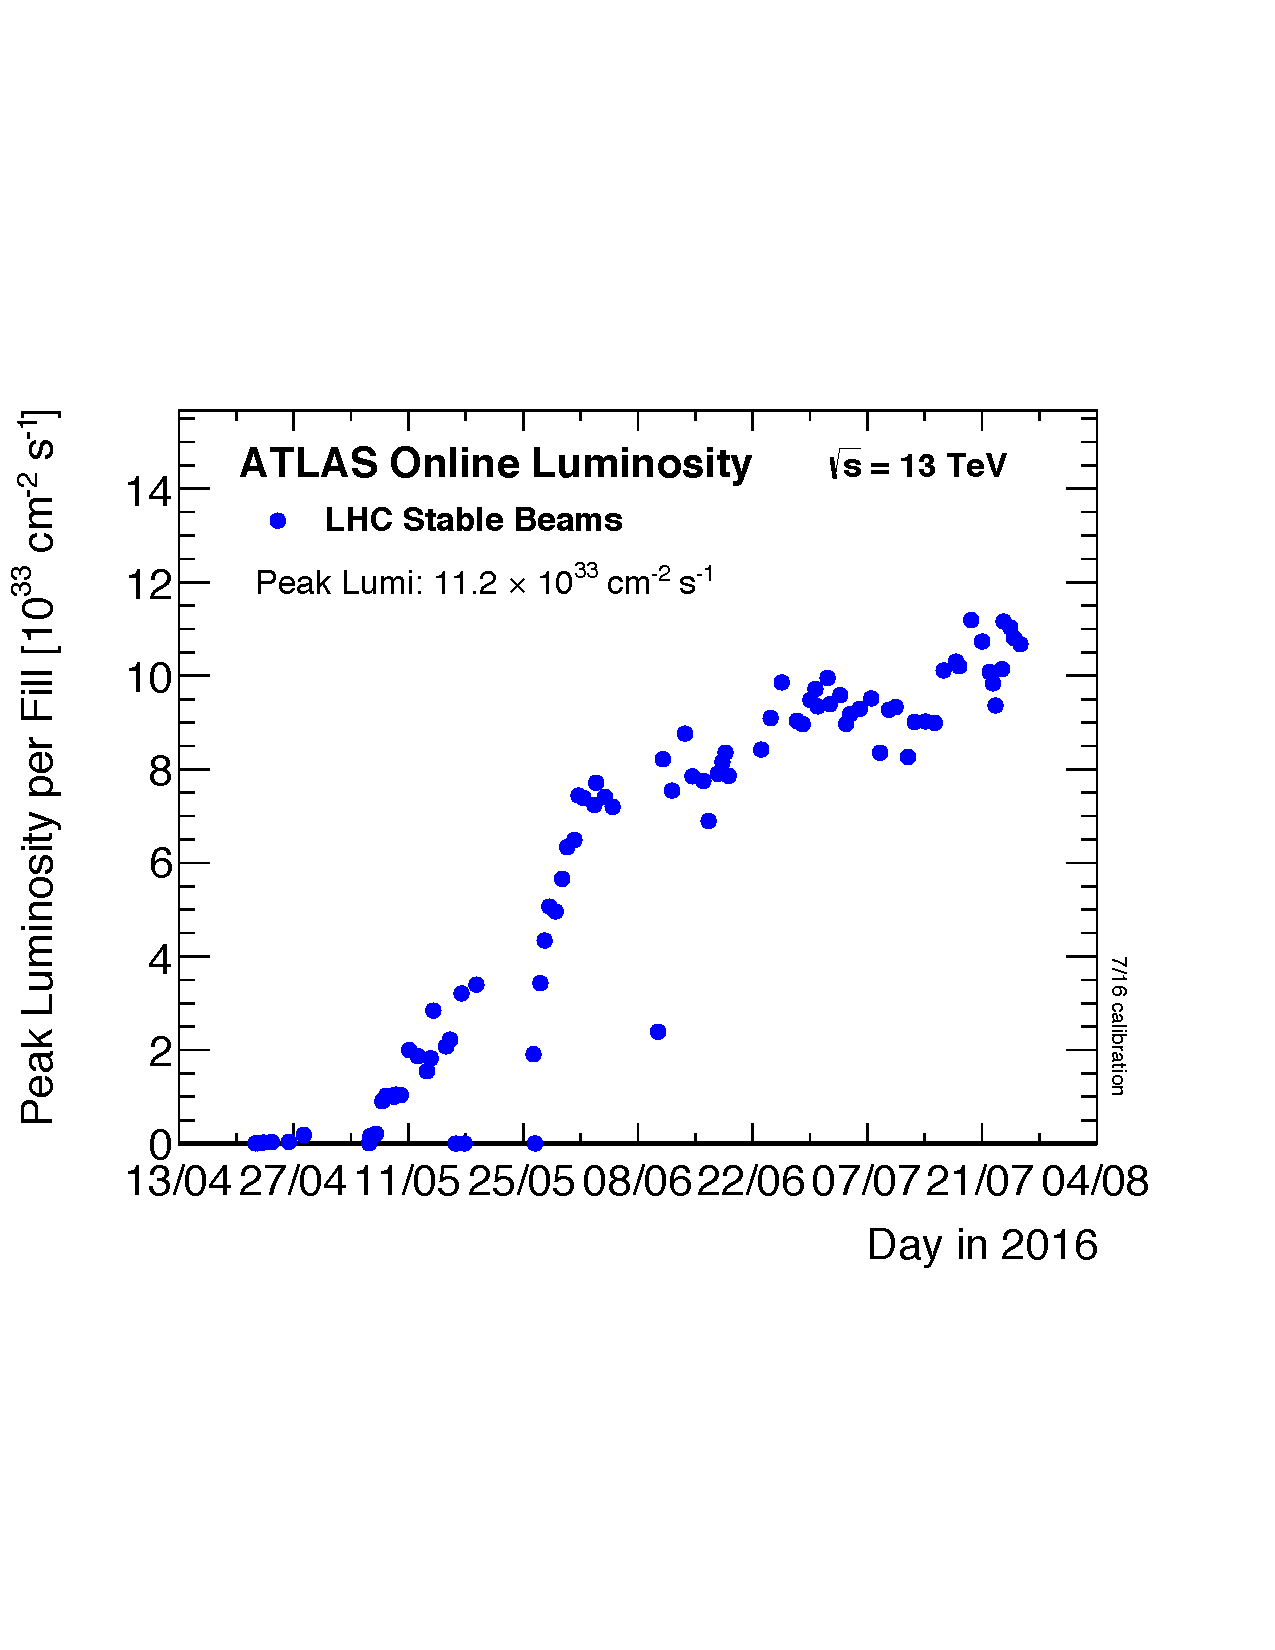
\includegraphics[width=\textwidth]{peakLumiByFill-1}
\end{subfigure}
\begin{subfigure}[t]{0.48\textwidth}
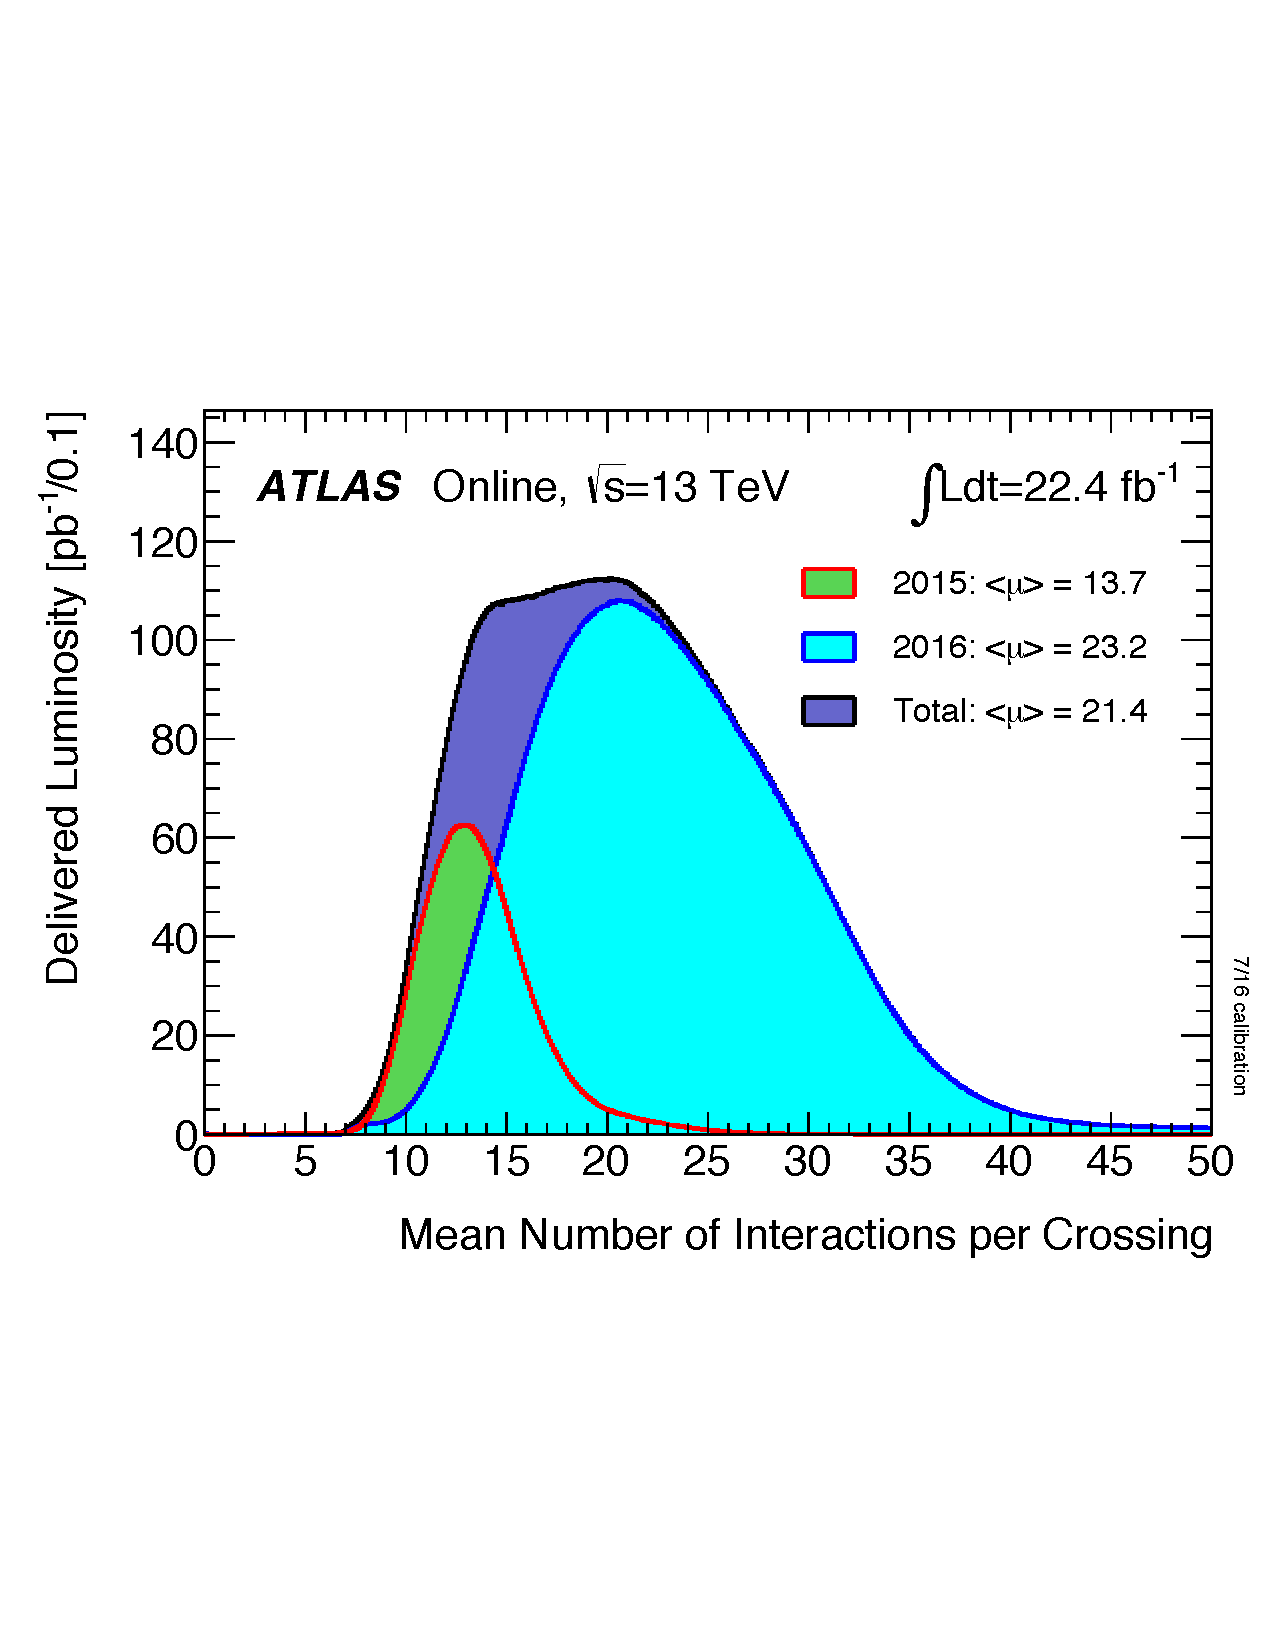
\includegraphics[width=\textwidth]{mu_2015_2016_ICHEP}
\end{subfigure}
\vspace{-2cm}
\caption{Run conditions during Run 2: ATLAS online luminosity (left), ATLAS online pileup (right) \cite{atlasTwiki}.}
\label{fig:lumi_pileup_1}
\end{figure} 
The L1 accept 
rate has also increased from 75 kHz in Run 1 to 100 kHz in Run 2 and the average output rate of the data logger system has 
increased from 400-600 Hz in Run 1 to about 3 kHz with 1.5 kHz for physics data. 
%of which is from the 1.5 kHz for an event size of 1.5 MB. 
Moreover, there were new detectors that were added in Run 2
(Insertable B-layer (IBL), L1 topological trigger, Fast Tracker (FTK))\cite{Aad:1602235} leading to 
an increase of 20\% in the number of readout channels. 
To be able to deliver more rate to the High Level Trigger (HLT), the upgrade also targeted the Readout System (ROS)\cite{PanduroVazquez2016939}. 
For the same reason the two level of the HLT system were collapsed into a single level which made the system more flexible 
 allowing for incremental data retrieval and analysis. 
The dataflow network system was re-designed to increase its capacity and simplify its architecture\cite{1742-6596-396-1-012033}.

%Given all these changes, the DAQ system needed an upgrade to satisfy the new requirements. In particular, the upgrade targeted the 
%replacement of the buffering hardware of the Readout System (ROS) to increase the readout rate \cite{PanduroVazquez2016939}, 
%the merging of the Region-of-Interest (RoI) 
%based selection with event building and filtering into a single process allowing incremental data collection and analysis in the 
%High Level Trigger (HLT), and a re-design of the network system connecting the ROS with the HLT to increase its capacity and simplify 
%its architecture \cite{1742-6596-396-1-012033}. 


\section{ATLAS Dataflow Design}

%The ATLAS data-taking proceeds in stages starting from the RoIs
%identified by the L1 triggers that are sent to the HLT for processing.
In Run 1, the farm was subdivided to several slices, with 
each slice managed by a dedicated supervisor. This layout has been 
dropped in favor of global management by a single farm master 
operating at 100 kHz referred to as the HLT supervisor (HLTSV). 
The Region of Interest Builder (RoIB) that assembles the RoIs
previously implemented on a VMEbus 
system is now integrated with the HLTSV and the RoI building done in software. 
%The architecture of the HLT has changed where the two levels of 
%the software trigger, known as Level 2 and the Event Filter, that were each 
%running on separate farms were merged into 
%a single farm with an increased number of available cores. 
The change in the HLT architecture from two to one level
required re-writing the HLT software and algorithms in such a way that 
each node in the farm can perform all processing steps. The handling of these
processing steps is done by a single Data Collection Manager (DCM) process 
running on each HLT node to manage the L1 RoIs, the dataflow 
between the ROS and the HLT processing units (HLTPU), 
the event building processes, and the data logging.
 In the new architecture, the computing resources are managed more efficiently
by balancing the utilization of all cluster nodes depending on the active HLT 
algorithms and by sharing the HLT code and services to reduce memory and 
resource usage. 

The dataflow network was simplified and upgraded to handle a larger data volume.
A single network is used for 
RoI based access from the ROS, event 
building in the HLT processing nodes, and sending data for logging. 
A 10 GbE connectivity has been adopted throughout  the dataflow system
resulting in a factor of four increase in bandwidth between the data loggers and
the permanent storage, and a 4$\times$10 GbE output from each ROS PC to the core routers. 
The HLTSV and the HLT racks are all connected directly to each of the two core routers via 
 2$\times$10 GbE connection. Each HLT rack is hosting up to 40 nodes connected by 2$\times$1 GbE to the top-rack switches. 
The capacity of the routers can accommodate
an increase in the number of HLT server racks and ROS PCs by a factor of two, 
which will be needed when the system scales as run conditions 
change. The core routers also provide load balancing and traffic shaping protocols \cite{1742-6596-396-1-012033}
to distribute the data throughout the system more evenly. A duplication of core routers provide link redundancy at every level in 
case of link or switch failures.


%\begin{figure}[t!]
%\centering
%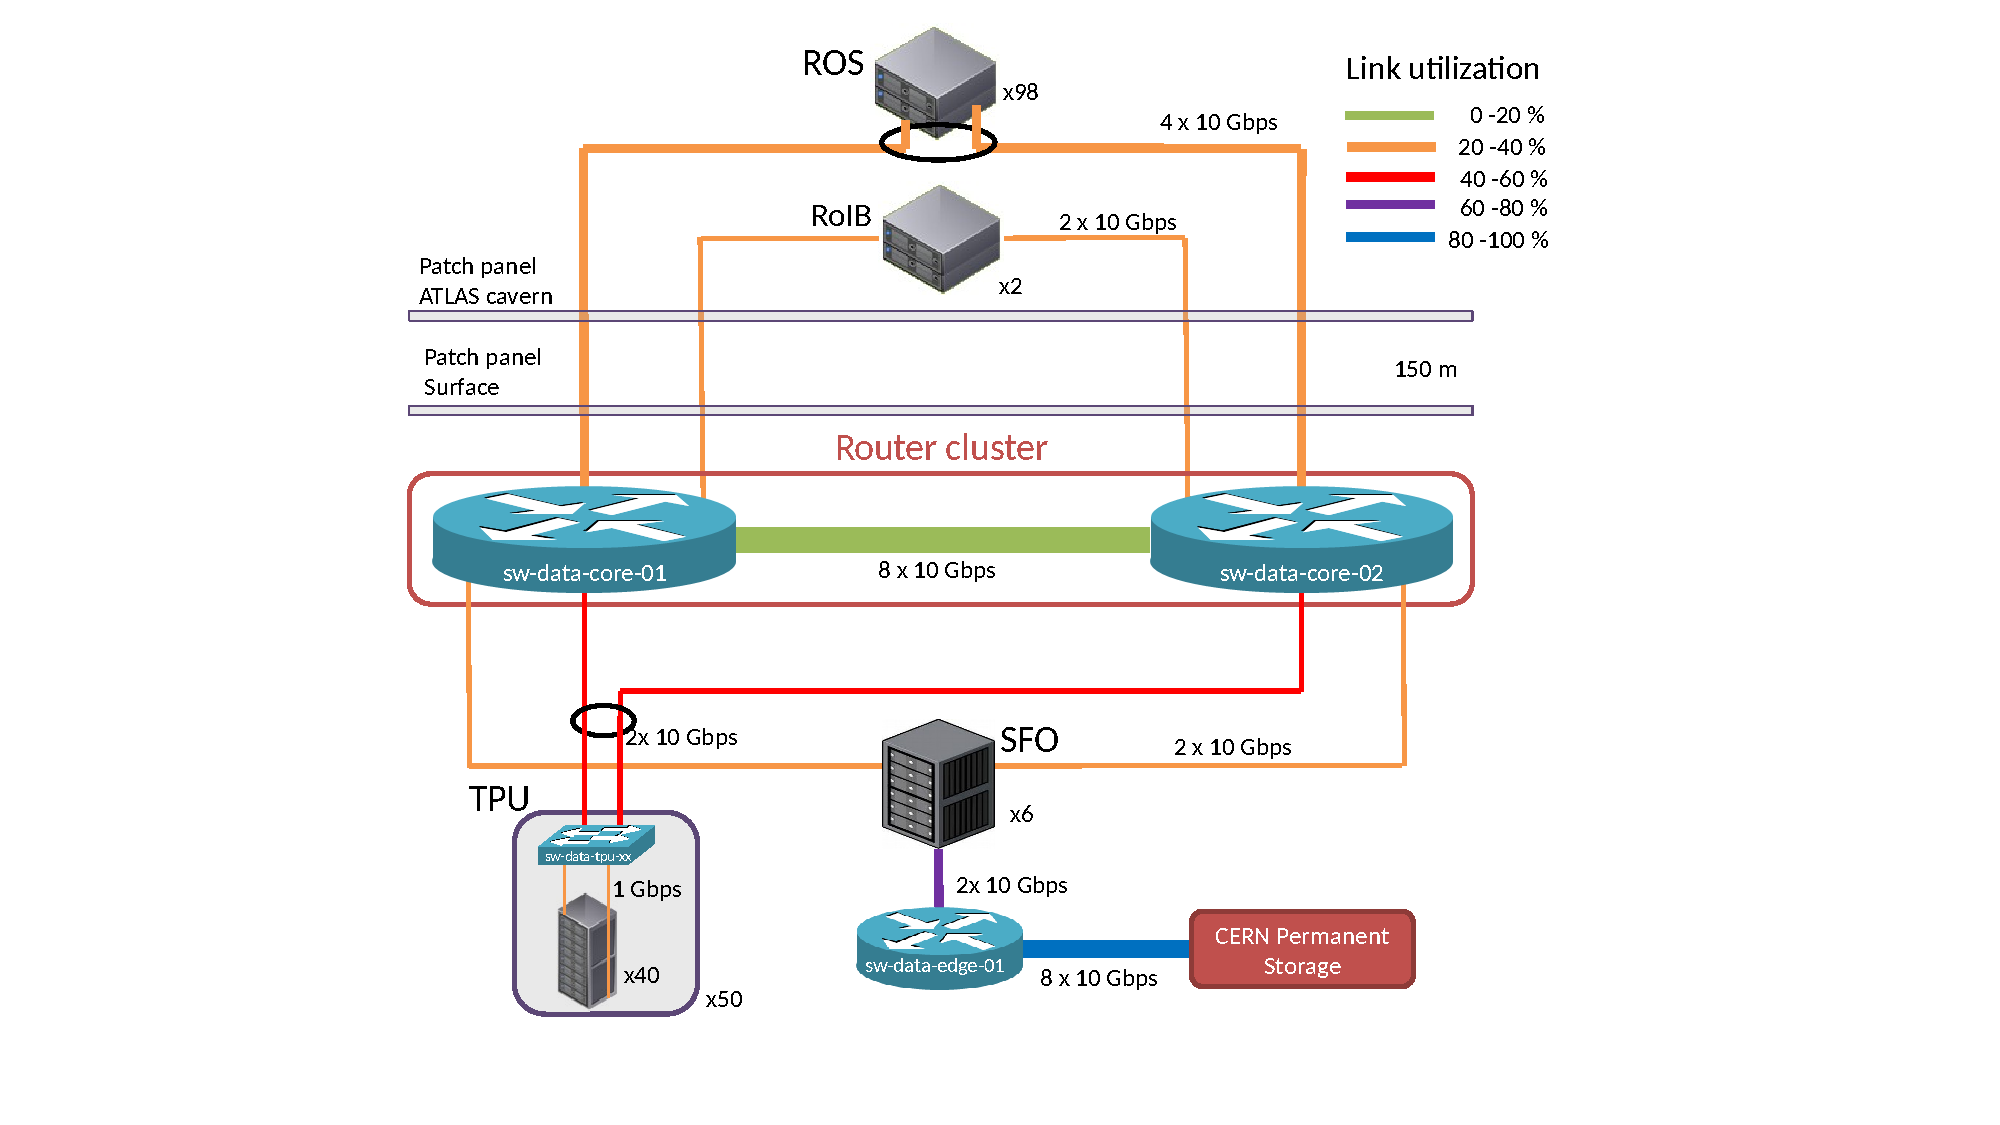
\includegraphics[width=1.2\textwidth]{network} 
%\vspace{-1cm}
%\caption{ATLAS Dataflow network}
%\label{fig:tdaq_diagram}
%\end{figure} 

To take advantage of multi-core architectures, the dataflow
 software is using multi-threaded software design for CPU consuming operations.
The Input/Output of the dataflow is based on asynchronous communication using industry standard libraries
such as the Boost::ASIO library. All the ATLAS software suite was switched to exclusively 64 bit operation in 2016.



%In summary, the elements of the Run 2 ATLAS dataflow are:

%\begin{itemize}
%\item The Readout Sytem (ROS) buffers front-end data from the detectors and provides a standard interface to the DAQ system.
%\item The Region of Interest Builder (RoIB) receives teh L1 trigger information from the RoIs and combines the information for the HLT supervsior.
%\item The HLT Supervisor (HLTSV) can handle the input from the RoIB and manage the HLT farm of about 2000 machines at over 100 kHz.
%\item The Data Collection Manager (DCM) handles all Input/Output on the HLT nodes, including RoI requests from the HLT and full event building.
%\item The HLT processing units (HLTPU) run the actualy HLT algorithms which 
%are forked from a single mother process to maximize memory sharing.
%\item The Data loggers or SubFarm Output (SFO) are responsible for savind the 
%accepted events to disk, and sending the files to CERN permanent storage infrastructure.
%\end{itemize}


\begin{figure}[!t]
\centering
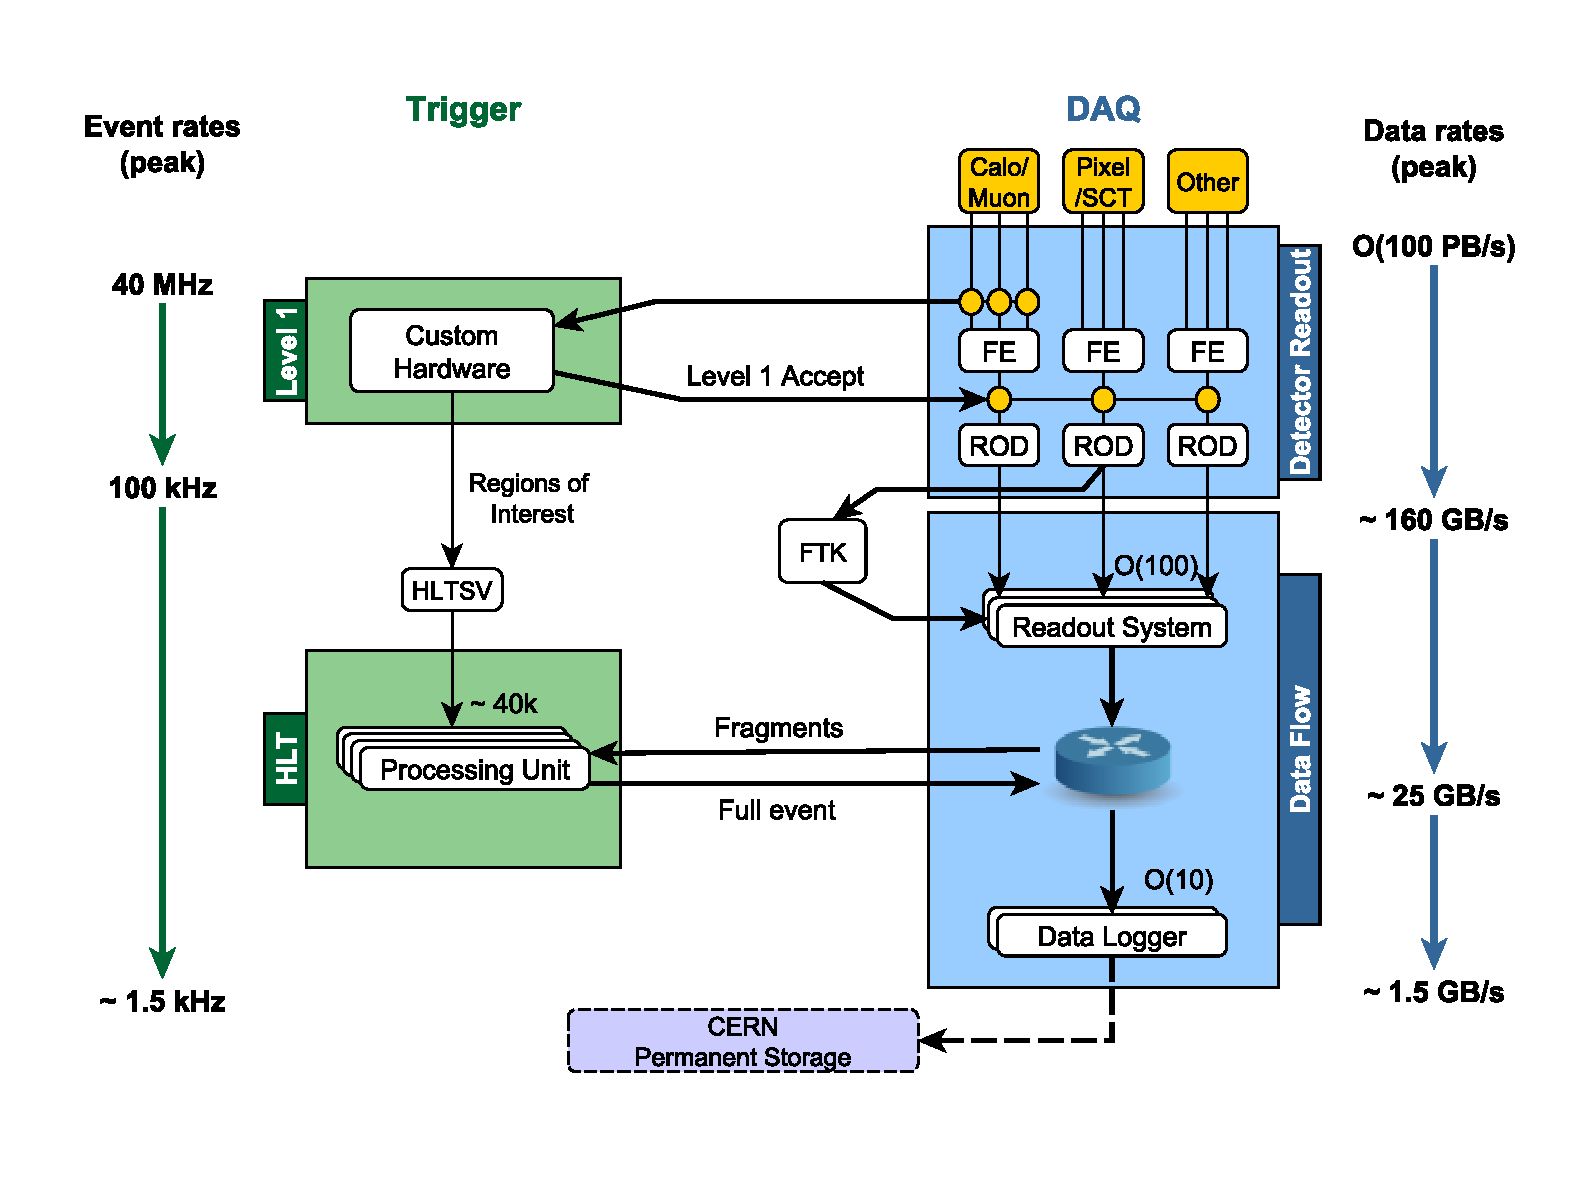
\includegraphics[width=0.75\textwidth]{tdaqFullNew2016}
\vspace{-0.5cm}
\caption{ATLAS TDAQ architecture.}
\label{fig:tdaq_diagram}
\end{figure} 

\section{Region of Interest Builder}

The first step of the HLT processing is to run on the RoIs found by the L1 hardware trigger. These
RoIs are collected and distributed to the HLT farm by the RoIB \cite{1748-0221-11-02-C02080} which was the 
latest change to the ATLAS dataflow. 
%This system was installed in ATLAS
% between the 2015 and 2016 data taking periods. 
The
evolution of the RoIB system from a crate of custom VME-based electronics (VME-RoIB) to a commodity
PC hosting a custom PCI-Express card (PC-RoIB) has been undertaken to increase the system performance,
flexibility, and ease of maintenance. The functionality of the VME-RoIB previously possible only in FPGAs has
now been implemented in a multi-threaded C++ software library. 
For each proton-proton collision that is accepted by the L1 trigger, the
RoIB receives an RoI record from the custom inputs via S-Link. The RoIB assembles these records into
a single record which is then forwarded to the HLTSV. The HLTSV then
distributes these single records to the HLT farm. The RoIB is also responsible for monitoring the
data integrity of the incoming fragments and diagnostic performance of the system.

As shown in Figure \ref{fig:roib_summary}, the performance of the PC-RoIB with realistic running ATLAS conditions
is improved over the VME-RoIB particularly at high RoI sizes. 

\begin{figure}[t!]
\centering
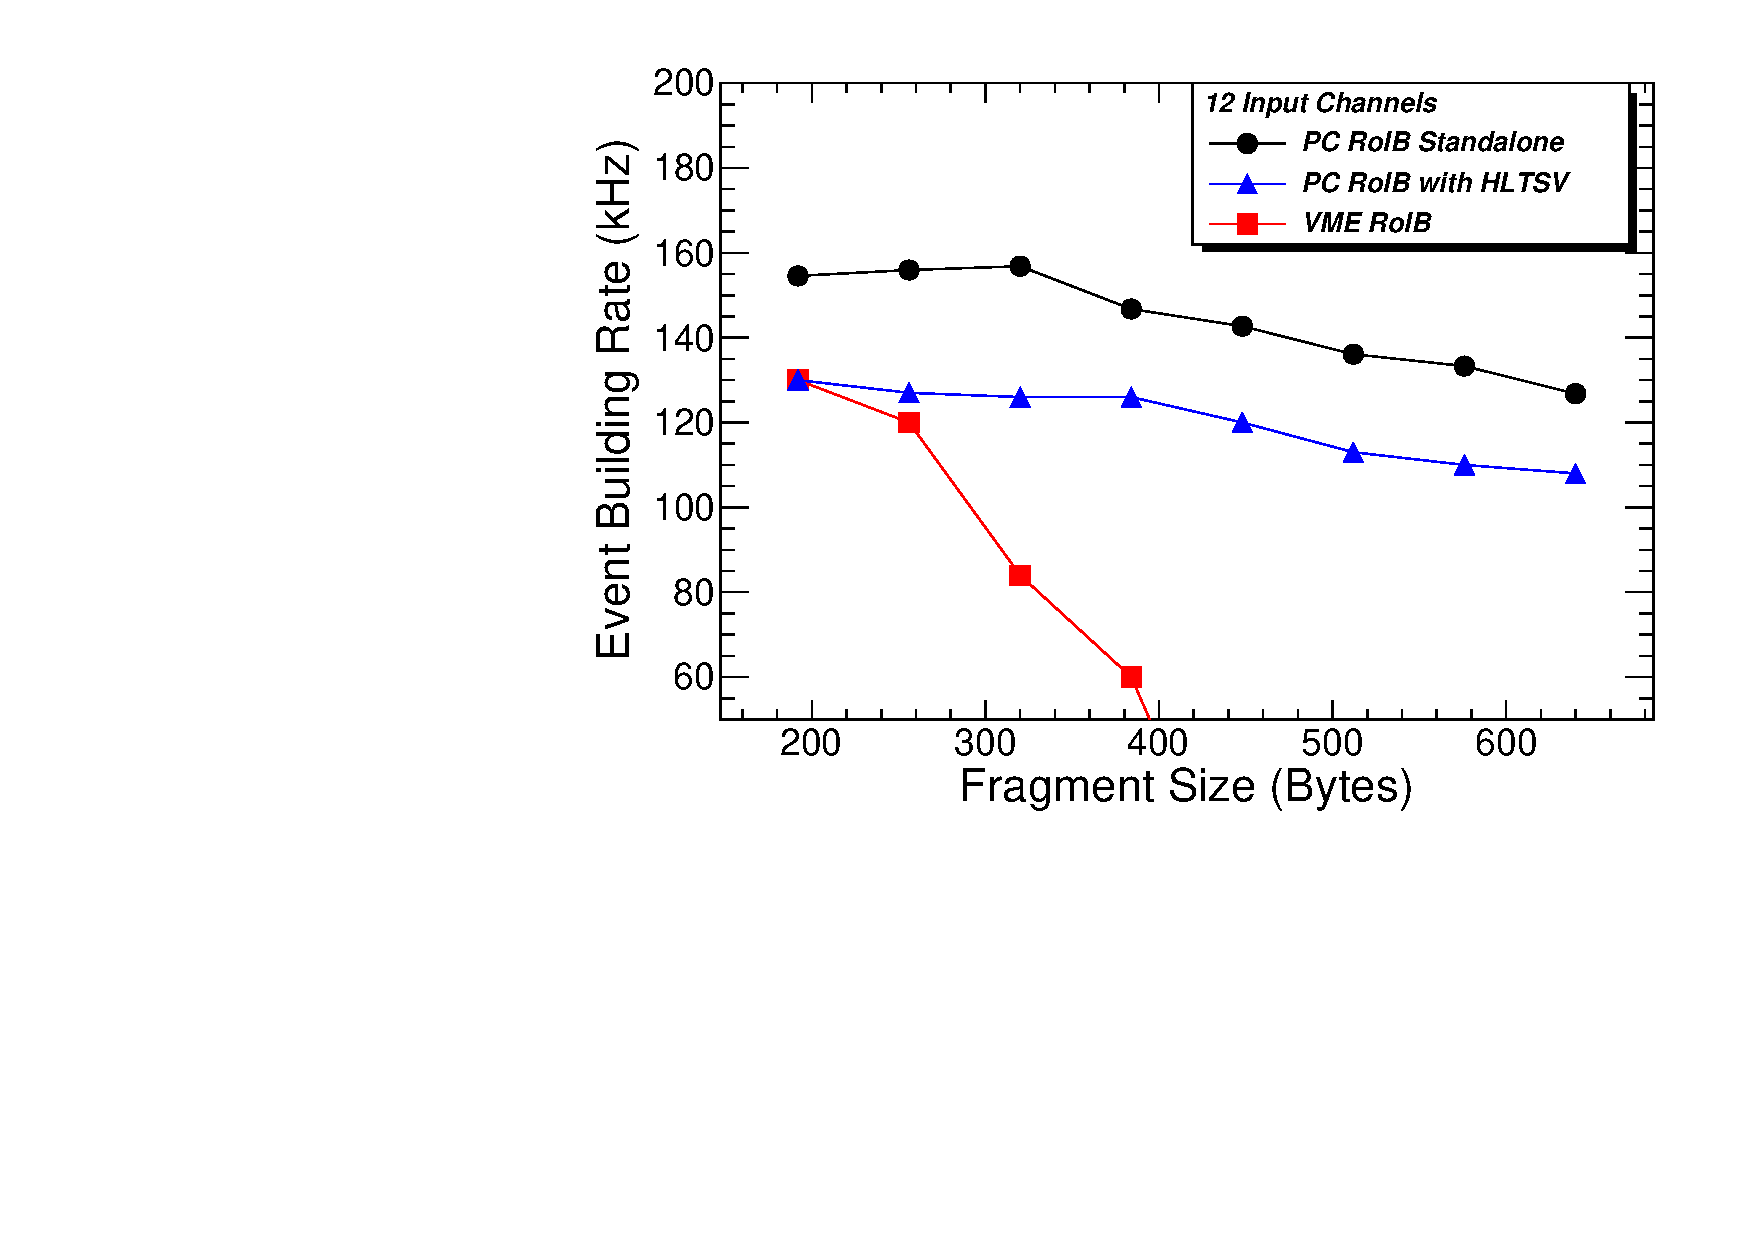
\includegraphics[width=0.5\textwidth]{roib_summary_size} 
\caption{The event building rate as a function of the RoI record size in Bytes. The rates are shown for a standalone application that implements 
a minimal interface for event building, the integrated RoIB software into an HLTSV process
running within the full ATLAS TDAQ software suite, and for comparison the VME-RoIB performance.}
\label{fig:roib_summary}
\end{figure} 

Figure \ref{fig:roib_pileup_l1rate} shows that the memory usage of the HLTSV is at the level of 5\% and that the RoIB event assembly does not depend 
on pileup conditions.


\begin{figure}[t!]
\centering
\begin{subfigure}[t]{0.48\textwidth}
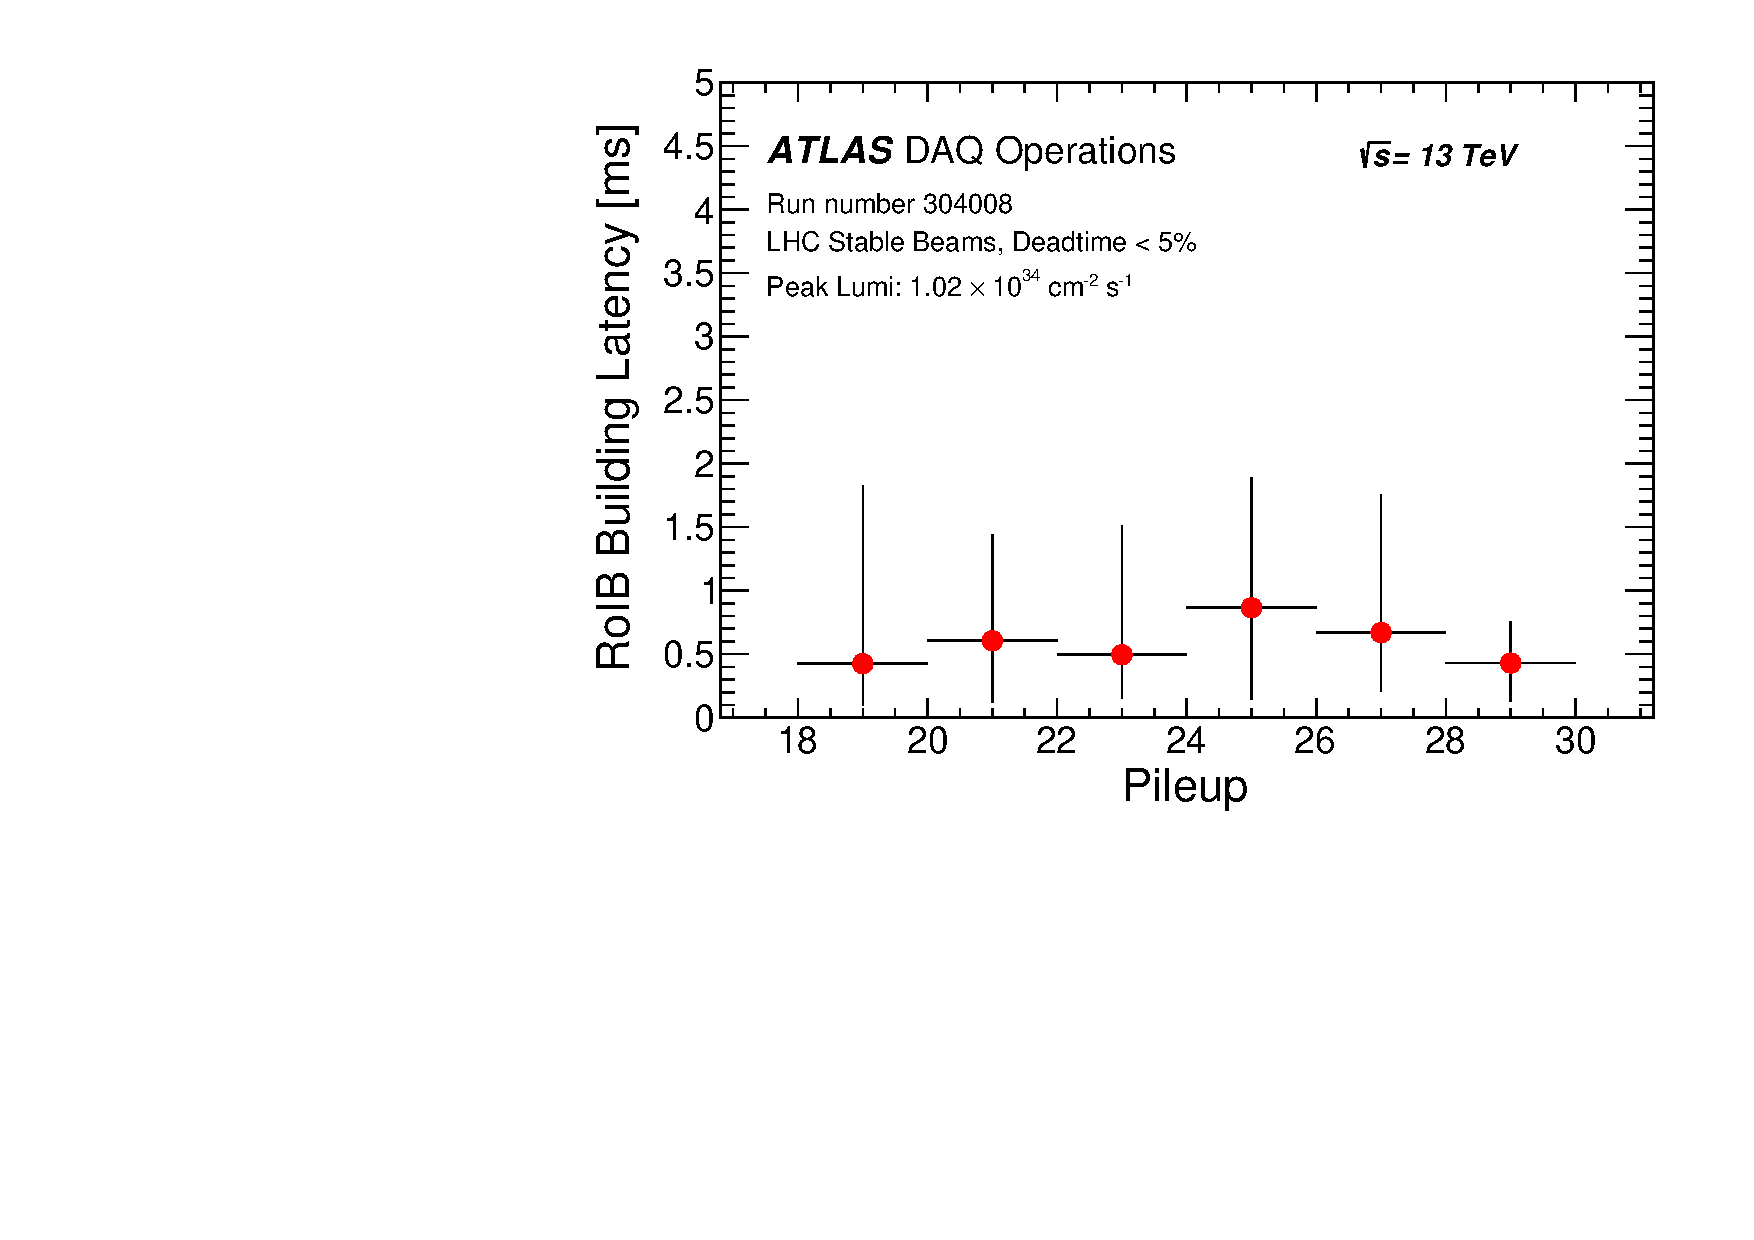
\includegraphics[width=0.95\textwidth]{GrAssym_run_304008_pileup_RoIBbuildtime}
\end{subfigure}
\begin{subfigure}[t]{0.48\textwidth}
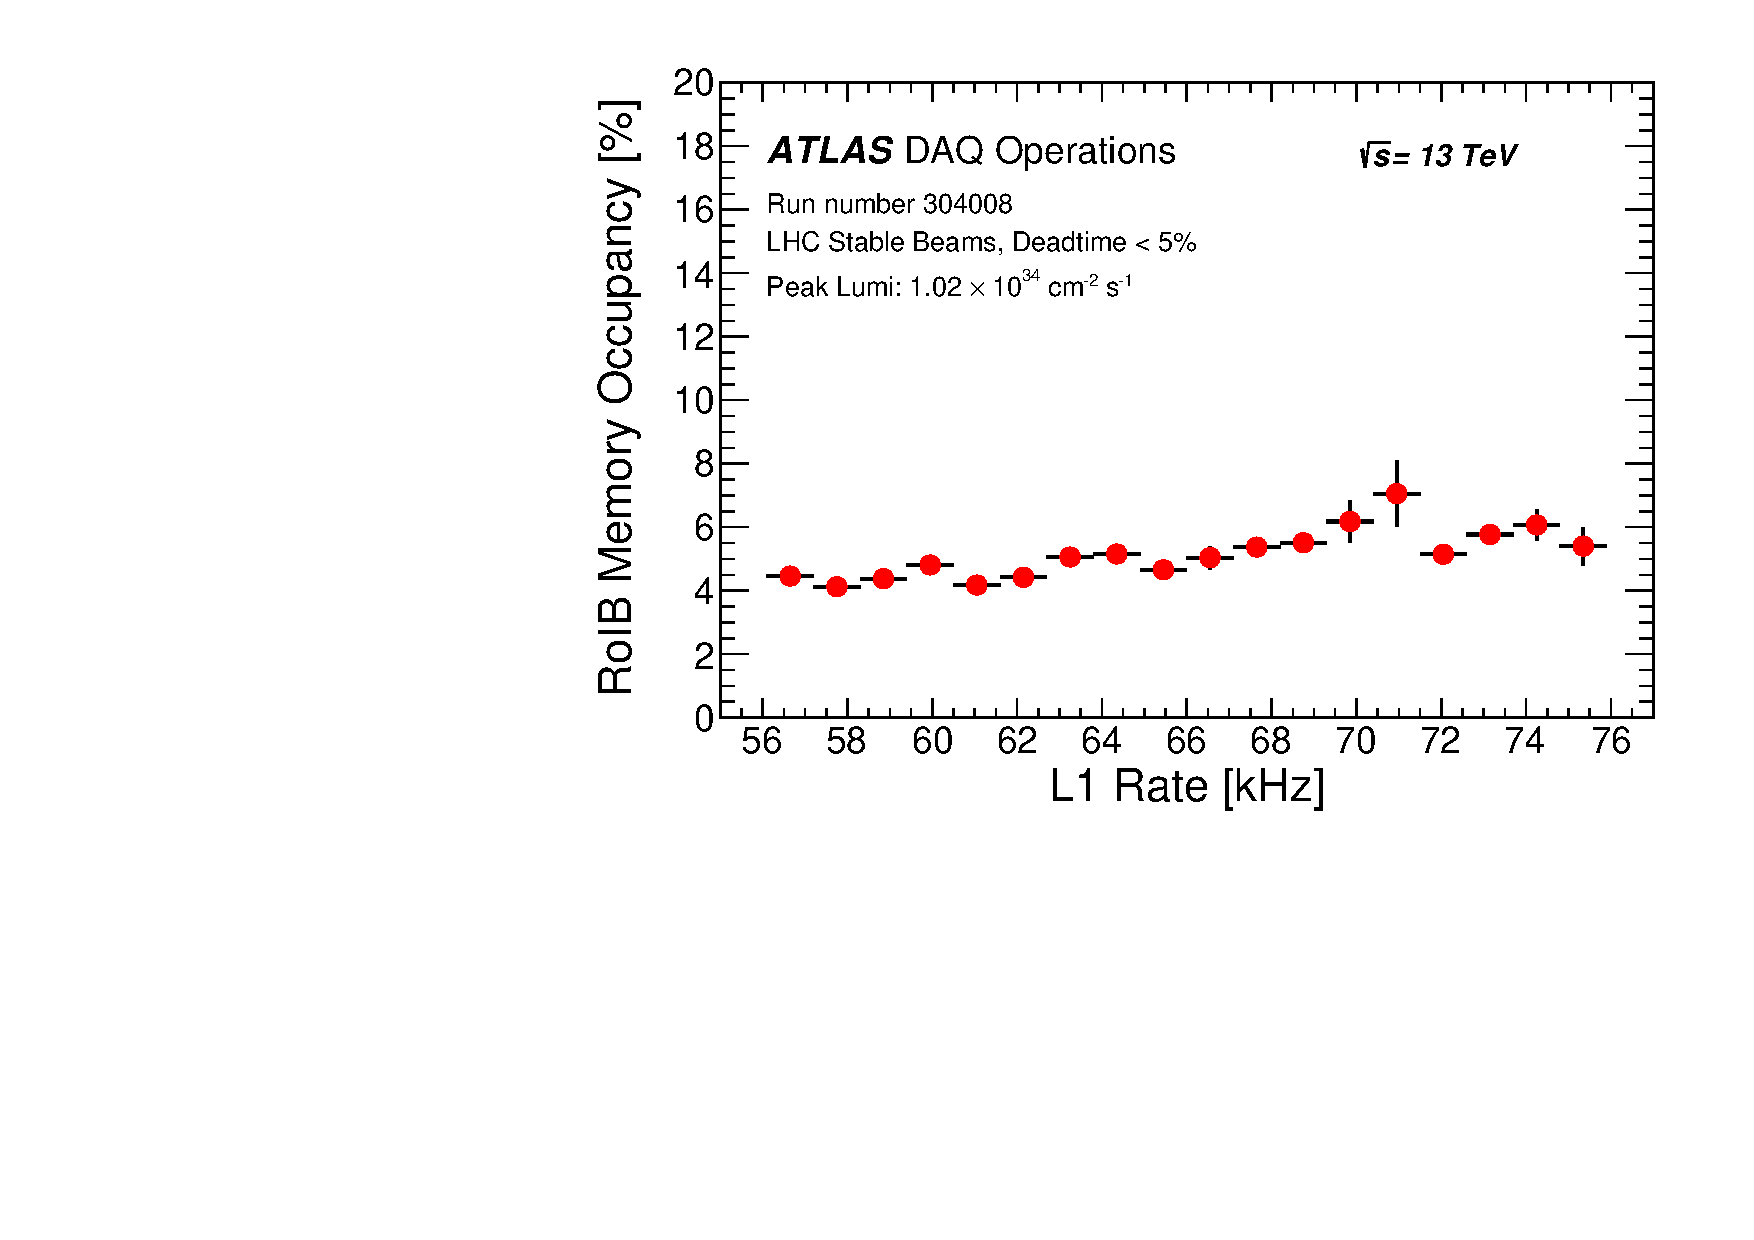
\includegraphics[width=0.95\textwidth]{hProf_run_304008_l1rate_RoIBMemOccup}
\end{subfigure}
\vspace{-0.25cm}
\caption{RoIB performance: RoIB building latency as a function of pileup (left), RoIB memory occupancy as a function of L1 rate (right).}
\label{fig:roib_pileup_l1rate}
\end{figure} 


%The initial tests were
%performed with a standalone application that implements a minimal interface for event building.
%Once the system was validated, the relevant code modules were integrated into an HLTSV process
%running within the full ATLAS TDAQ software suite with appropriately scaled test hardware to
%represent the remaining elements of the system.

%\section{Dataflow Network}

\section{Performance in Run 2}

The reliable operation of the TDAQ system directly impacts the efficiency of the ATLAS experiment 
in recording the collisions delivered by the LHC. As a result, high data-taking efficiency is crucial 
for the ATLAS physics program.
The ATLAS recorded efficiency in 2016 is over 90\%, as shown in Figure \ref{fig:tdaq_diagram} with a negligible fraction of data 
loss due to 
the DAQ system. The new dataflow architecture is scaling well with the increased 
instantaneous luminosity during 2016 data-taking and is capable of handling larger pileup and thus larger event sizes.
For illustration,  Figure \ref{fig:run_pileup} shows the evolution of the average processing time per event and 
the event size where there is relatively mild increase as a function of pileup which will within the system capacity.

\begin{figure}[t!]
\vspace{-0.5cm}
\centering
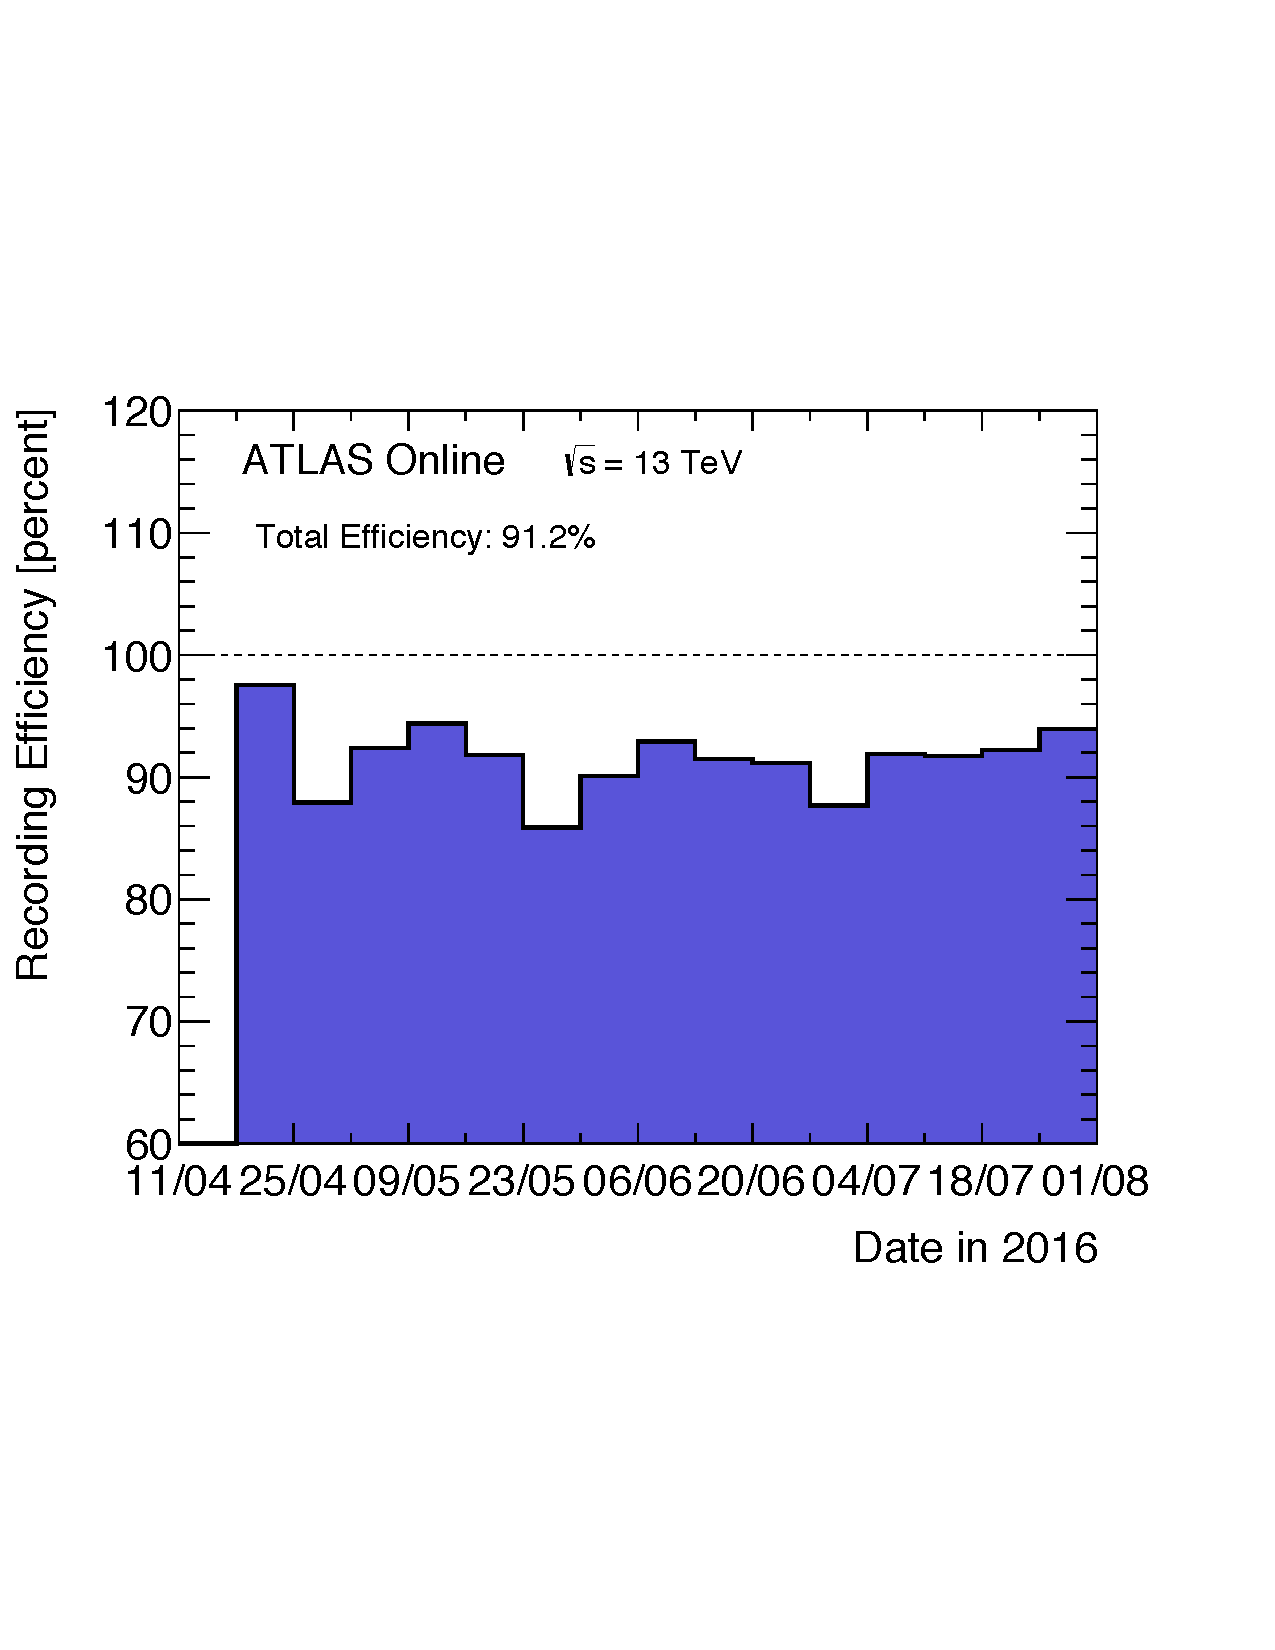
\includegraphics[width=0.5\textwidth]{recEffByWeek-1} 
\vspace{-2.5cm}
\caption{ATLAS recorded efficiency \cite{atlasTwiki}.}
\label{fig:tdaq_diagram}
\end{figure} 


\begin{figure}[t!]
%\vspace{-0.1cm}
\centering
\begin{subfigure}[t]{0.48\textwidth}
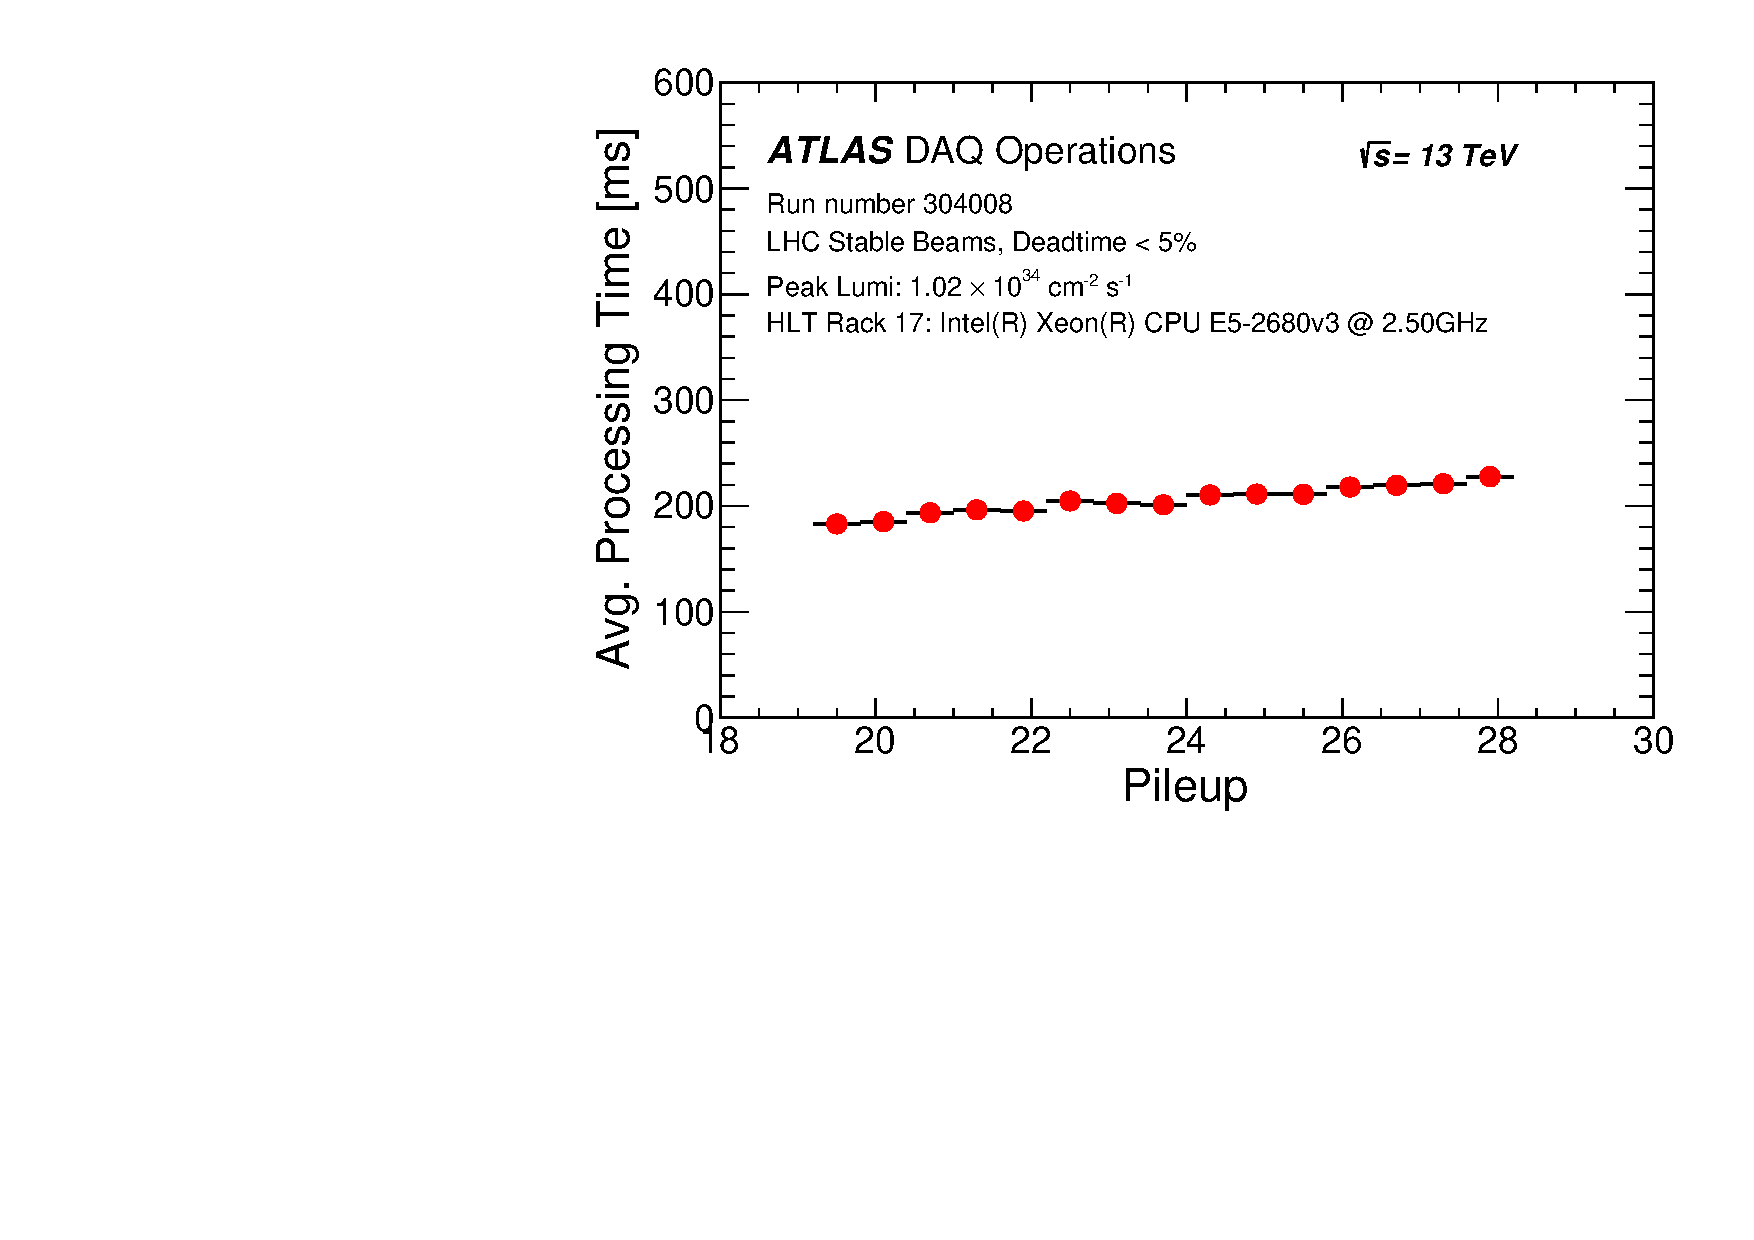
\includegraphics[width=.95\textwidth]{hProf_run_304008_pileup_AvgProcessingTime.pdf}
\end{subfigure}
\begin{subfigure}[t]{0.48\textwidth}
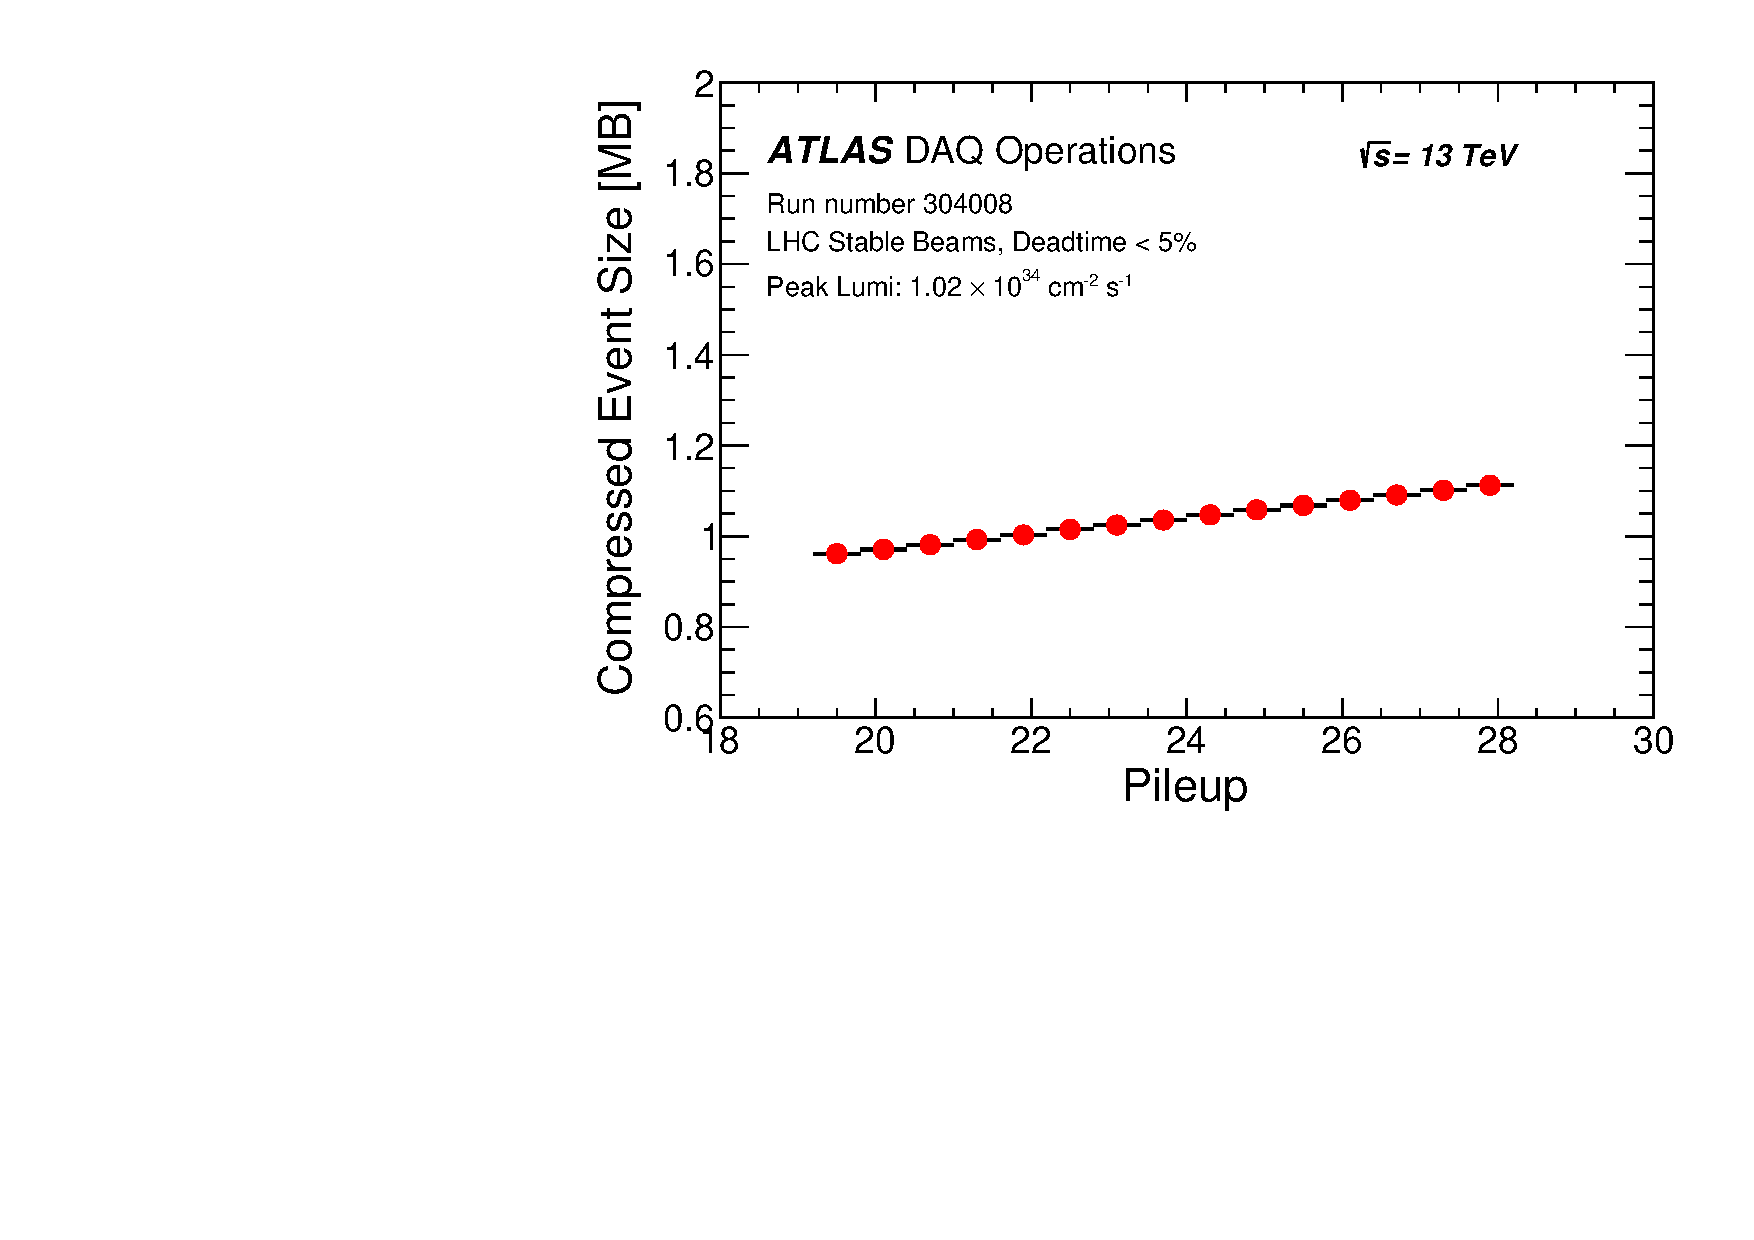
\includegraphics[width=.95\textwidth]{hProf_run_304008_pileup_EventSize.pdf}
\end{subfigure}
\vspace{-0.3cm}
\caption{Performance in Run 2: Average processing time as a function of pileup (left), compressed event size as a function of pileup (right).}
\label{fig:run_pileup}
\end{figure} 

\section{Conclusion}

The dataflow system of ATLAS was re-shaped for Run 2 in order to handle the 
 more demanding run conditions expected throughout the run. The new redesign 
profitted from the technological progress 
that took place in the last few years. As a result, the new system 
is considerably simplified, more performant, and scalable. Moreover,
there is more headroom in performance to cope with more challenging run conditions
of the LHC to ensure that ATLAS DAQ continues delivering physics data with high efficiency. 


\section{Introduction}\label{sec:intro}

The ATLAS \cite{atlas} detector's data acquisition system, illustrated in Figure \ref{fig:atlas_tdaq}, makes use of a multi-tiered trigger to reduce 
bandwidth from the LHC proton bunch crossing rate of 40 MHz
to the \\1 kHz written to disk \cite{evolution}. The first tier (Level-1 or L1) \cite{l1}, implemented in real time with custom electronics, 
makes an early event selection to determine if any objects of interest are present and reduces the data flow to 
100 kHz. The second tier, referred to as the High Level Trigger (HLT) \cite{hlt}, is implemented on a commodity computing cluster running custom triggering software. The HLT uses information from the
hardware based L1 system to guide the retrieval of information from the Readout System (ROS) \cite{ros}. 

Jet, electromagnetic and tau clusters, missing transverse momentum ($E_{\mathrm{T}}^{\mathrm{miss}}$), $\sum E_{\mathrm{T}}$, 
jet $E_{\mathrm{T}}$, and muon candidate information from L1 determine detector Regions of Interest (RoIs) that seed HLT processing. These RoIs are provided to the HLT by a custom VMEbus based system, referred to as the Region of Interest Builder (RoIB) \cite{vme_roib}.
The RoIB collects data from L1 
trigger sources and assembles the data fragments into a complete record of L1 RoIs. These RoIs are made available to the HLT to initiate event processing. In order to improve maintainability and scalability, and to minimize the amount of custom hardware needing to be supported, 
the RoIB will be implemented using commodity server hardware and an interface technology already deployed 
within the ATLAS Trigger and Data Acquisition (TDAQ) system. The approach of implementing the RoIB functionality in software has been investigated in the past 
and the conclusion at that time was that a software based approach is possible but requires a higher rate readout card \cite{swroib_past}. 
Since data readout cards operating at high rates became available and the capabilities of computers have improved with the increase 
in CPU clock speed and number of cores, it became possible to implement the RoIB functionality using a PC based approach. 
The PC based RoIB must duplicate the functionality of the VMEbus based RoIB which means that the PC based solution must receive and assemble the
individual L1 fragments, and pass them as a single L1 result to the HLT. Modern computers have multicore CPU architectures 
with the possibility of running multi-threaded application, a feature which is being fully exploited in the RoIB software to achieve 
the desired performance of 100 kHz over 12 input links for fragment sizes of 400 bytes.  
This paper describes the evolution of the RoIB from the VMEbus based system to the PC based system and gives details on the hardware, 
firmware, and software designs used to achieve the full RoIB functionality. 



\begin{figure}[tbp] % figures (and tables) should go top or bottom of
                    % the page where they are first cited or in
                    % subsequent pages
\centering
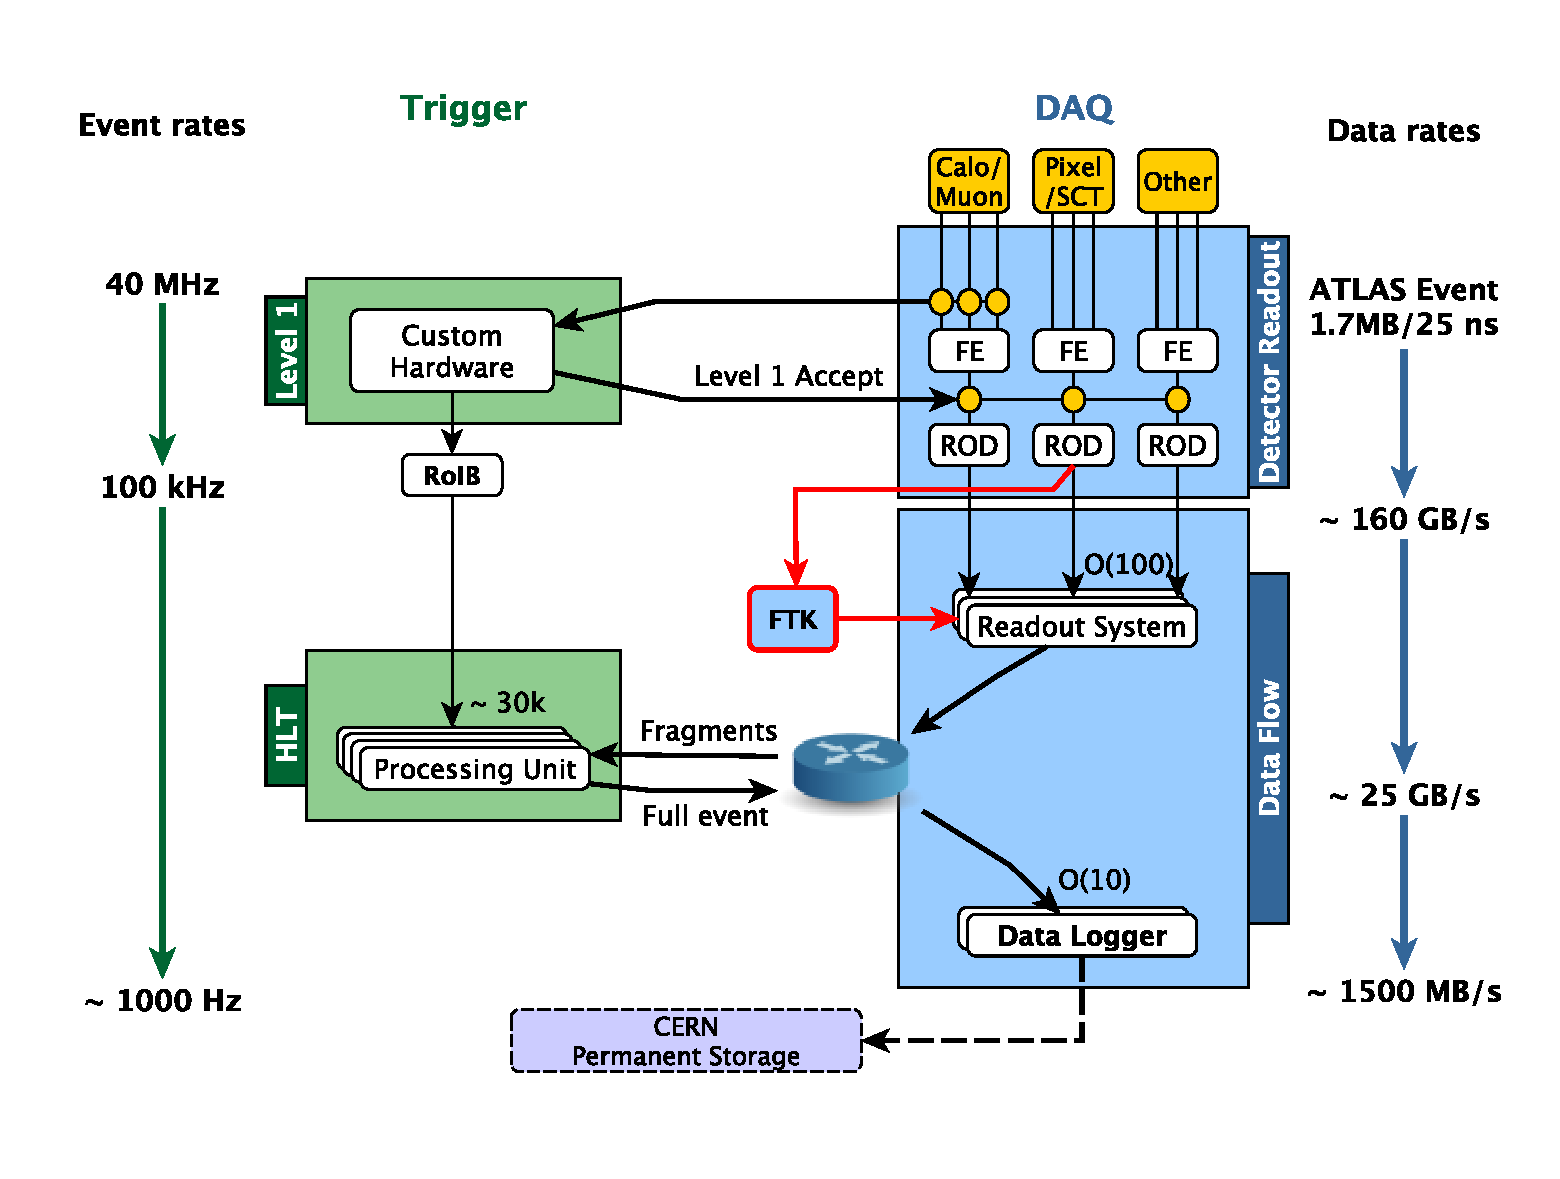
\includegraphics[width=.9\textwidth]{tdaqFullNew2015}
\caption{ATLAS TDAQ Architecture.}
\label{fig:atlas_tdaq}
\end{figure}



%\section{ATLAS TDAQ System }\label{sec:tdaq}

%\subsection{Challenges}\label{sec:tdaq_chal}

%\subsection{Architecture}\label{sec:tdaq_archi}


\section{VMEbus based RoIB}\label{sec:roib}

\subsection{Hardware implementation}\label{sec:roib_current}

The RoIB is implemented as a custom 9U VMEbus system that includes a controller which configures and monitors the system along with custom cards 
that receive and assemble the event fragments and send them to the HLT. Figure \ref{roib_run1} shows a block of the RoIB and 
its connection to external systems.
%\footnote{Note the L2 Supervisor farm from Run-1 has evolved to a commodity server PC running the HLTSV application.}.

\begin{figure}[tbp] % figures (and tables) should go top or bottom of
                    % the page where they are first cited or in
                    % subsequent pages
\centering
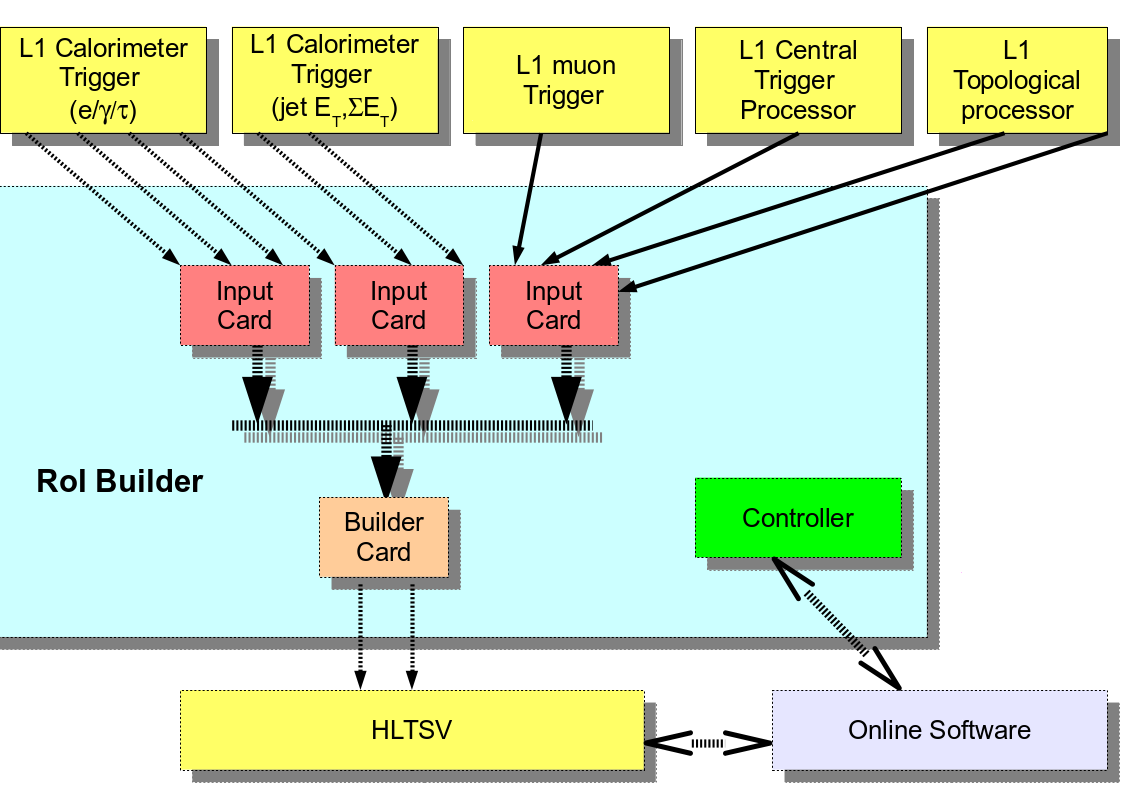
\includegraphics[width=.65\textwidth]{RoIB_context_v2.png}
\caption{Block scheme of the RoI Builder and overview of connections to external systems.  The
custom input and builder cards and the controller, a commercially available single board computer,
are installed in a single 9U VMEbus crate. The controller connects to the Control Network to interact with the rest of the 
data acquisition system.}
\label{roib_run1}
\end{figure}

The RoIB contains four input cards and uses one builder card in the Run-2 configuration. Each input card accepts three inputs from 
L1 subsystems. 
The builder card assembles the input data of the events and passes the results via two optical links 
to another receiver card in a PC running the HLT supervisor (HLTSV) application. The receiver card in the HLTSV is a TILAR card \cite{tilar}
 that implements four PCIe Gen1 lanes to interface with the two optical links. The HLTSV manages the HLT processing farm by using L1 results provided by the RoIB, retrieves events from the ROS, assigns events to HLT farm nodes, and handles event bookkeeping including requesting removal of data from ROS storage when no longer required. 

The fragments received by the RoIB are identified by a 32 bit identifier, the extended L1 ID (L1ID). 
The RoIB input cards use the L1ID and the number of outputs enabled to assign keys to the various fragments and send them to the output channel in the builder card that was 
assigned that key value. The input data is transferred over a custom J3 backplane. The backplane operates at 20 MHz and transfers 16 data bits per 
clock cycle simultaneously for up to 12 inputs. The total maximum data throughput is therefore 480 MB/s, 40 MB/s per input.  
The maximum size of any single fragment is limited to 512 bytes imposed by resources available in the FPGA firmware. The current RoIB input 
links are listed in Table \ref{tab:roib_links}.

\begin{table}[tbp]
\caption{L1 input sources to the RoIB.}
\label{tab:roib_links}
\smallskip
\centering
\begin{tabular}{|c|c|}
\hline
Source & Links\\
\hline
Central Trigger Processor (CTP)  & 1  \\
L1 calorimeters (e/$\gamma$, $\tau$, jet, $\sum E_\mathrm{T}$) & 6  \\
Muon Trigger to CTP Interface (MUCTPI) & 1  \\
Topological processor (L1Topo) & 2  \\
Spare & 2 \\
\hline
\end{tabular}
\end{table}

\subsection{System Performance and Evolution}\label{sec:roib_limit}

The custom VMEbus based RoIB operated reliably during the first run of the LHC, however, it is desirable to have a more flexible RoIB. 
In addition, the RoIB is getting close to its design limitation, as seen 
in Figure \ref{fig:cern_robinnproib}. For fragments of 400 bytes and inputs from eight L1 systems, referred to as channels, the current RoIB rate limit is 60 kHz which is below the required 100 kHz at 
L1. While the current fragment size coming from L1 are around 160 bytes, the sizes are expected to grow due to the increase of instantaneous 
luminosity and the complexity of L1 triggers. The current VMEbus system will be replaced by a PCI-express card hosted in the HLTSV PC with the 
possibility to upgrade the commodity hardware (e.g. ability to upgrade CPUs). 
The new configuration simplifies the readout architecture of ATLAS. The targeted rate for event building is 100 kHz over 12 input channels for 
fragment sizes in the order of 400 bytes.

\section{PC based RoIB}\label{sec:roib_new}

 A custom PCIe card developed by the ALICE collaboration, the Common ReadOut Receiver Card (C-RORC) \cite{alice}, was deployed as an 
upgraded detector readout interface within the ATLAS ROS with ATLAS specific firmware and software called the RobinNP \cite{crorc}. 
The new PC based RoIB uses the RobinNP firmware and a dedicated API to facilitate the implementation of the RoIB functionality 
on a commodity PC. In this section, we describe the C-RORC hardware as well as the RobinNP firmware, API, and the event building software. 
\subsection{The Common Readout Receiver Card}\label{sec:crorc}

The C-RORC implements 8 PCIe Gen1 lanes with 1.4 GB/s bandwidth to the CPU fed via 12 optical links each running 200 MB/s on 3 QSFP transceivers. It utilizes a single Xilinx Virtex-6 series FPGA that handles data input from the 12 links and buffers the data in two on-board DDR3 memories. It is also capable of processing and initiating DMA transfer of event data from the on-board memory to its host PC's memory. The major components of the C-RORC are annotated 
in the picture shown in Figure \ref{fig:crorc}.


\begin{figure}[tbp] % figures (and tables) should go top or bottom of
                    % the page where they are first cited or in
                    % subsequent pages
\centering
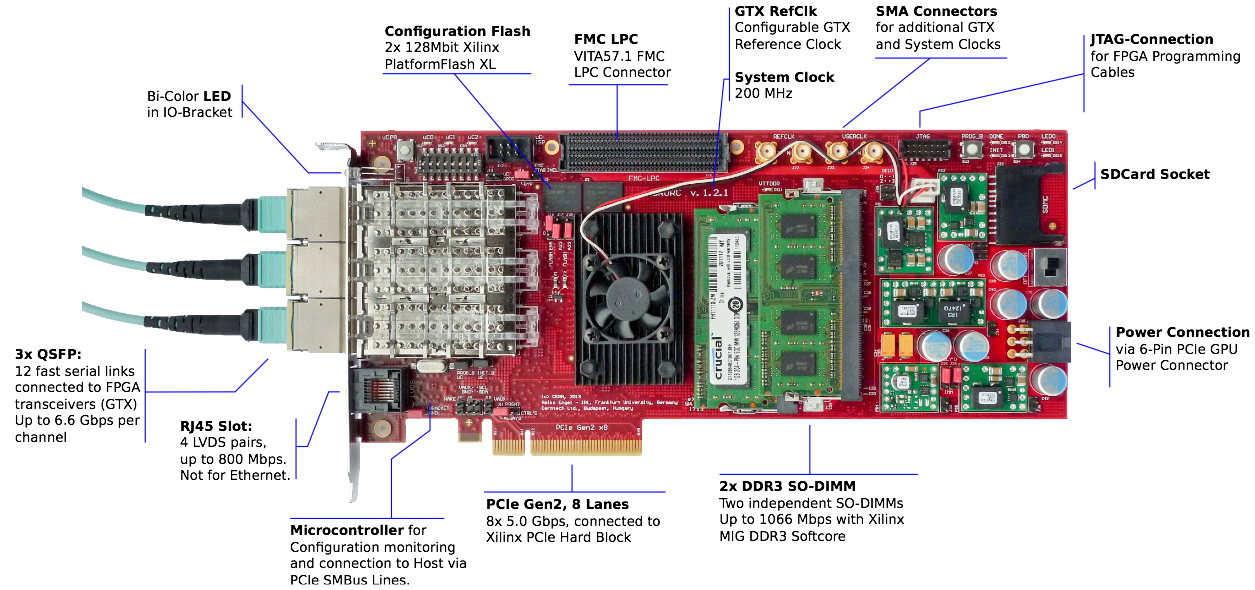
\includegraphics[width=\textwidth]{crorc.png}
\caption{Photo of the C-RORC board with the major components and features annotated \cite{crorc}.}
\label{fig:crorc}
\end{figure}

\begin{figure}[tbp] % figures (and tables) should go top or bottom of
                    % the page where they are first cited or in
                    % subsequent pages
\centering
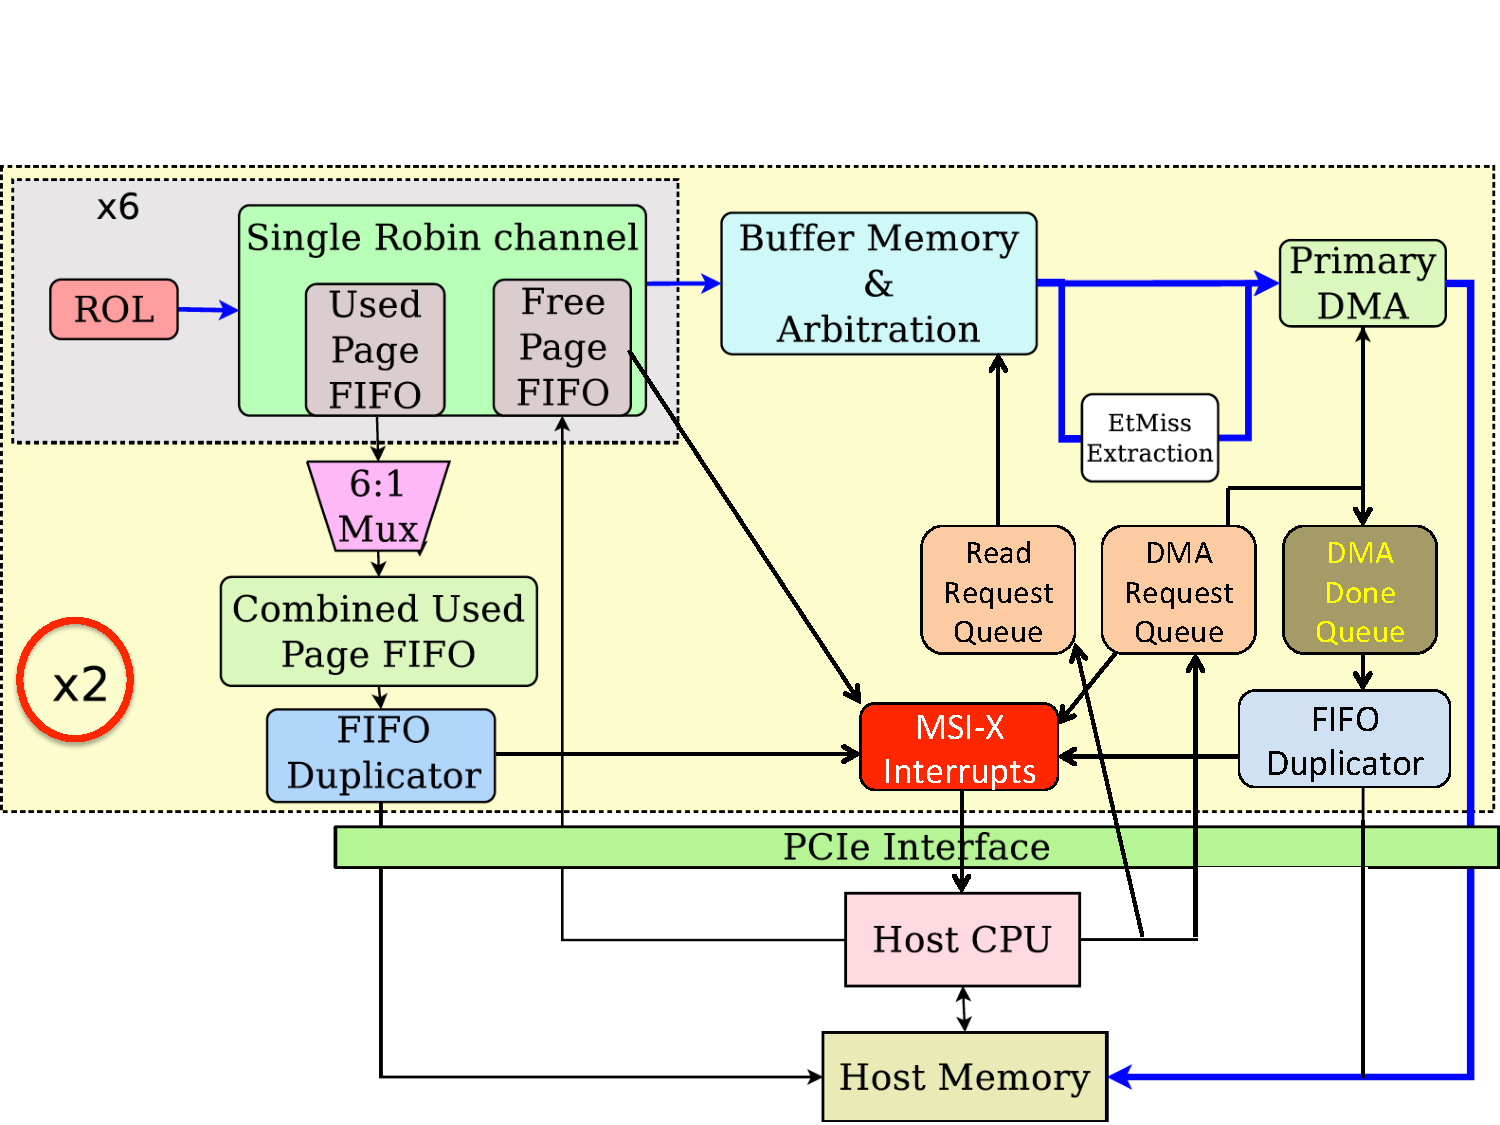
\includegraphics[trim = 0cm 0cm 0cm 2.5cm, clip, width=.71\textwidth]{RobinNP_Firmware}
%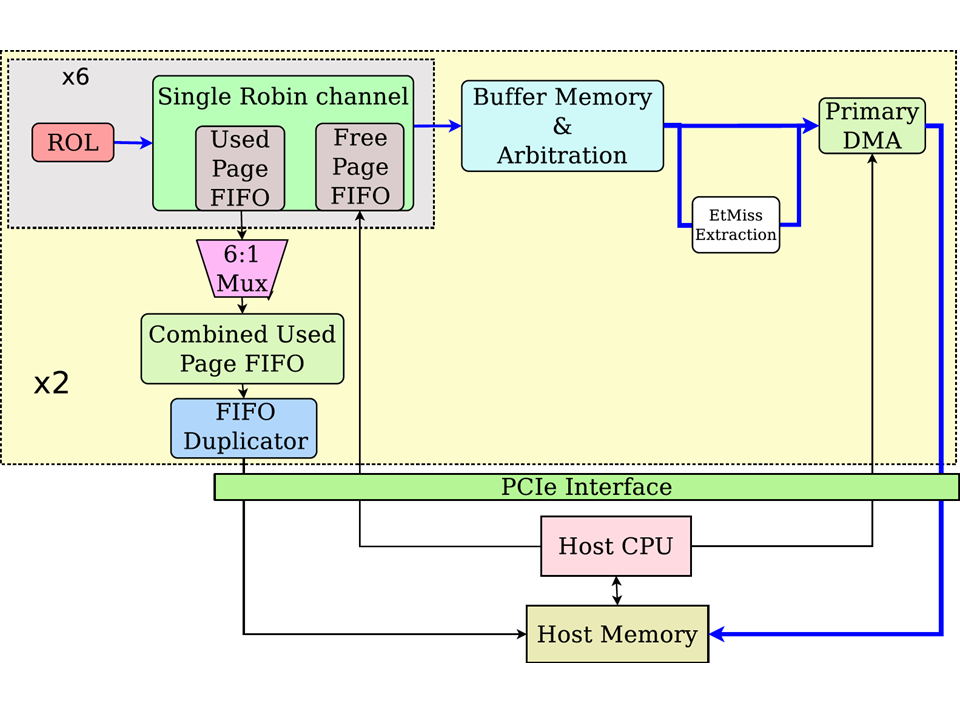
\includegraphics[width=.6\textwidth]{Firmware.jpg}
%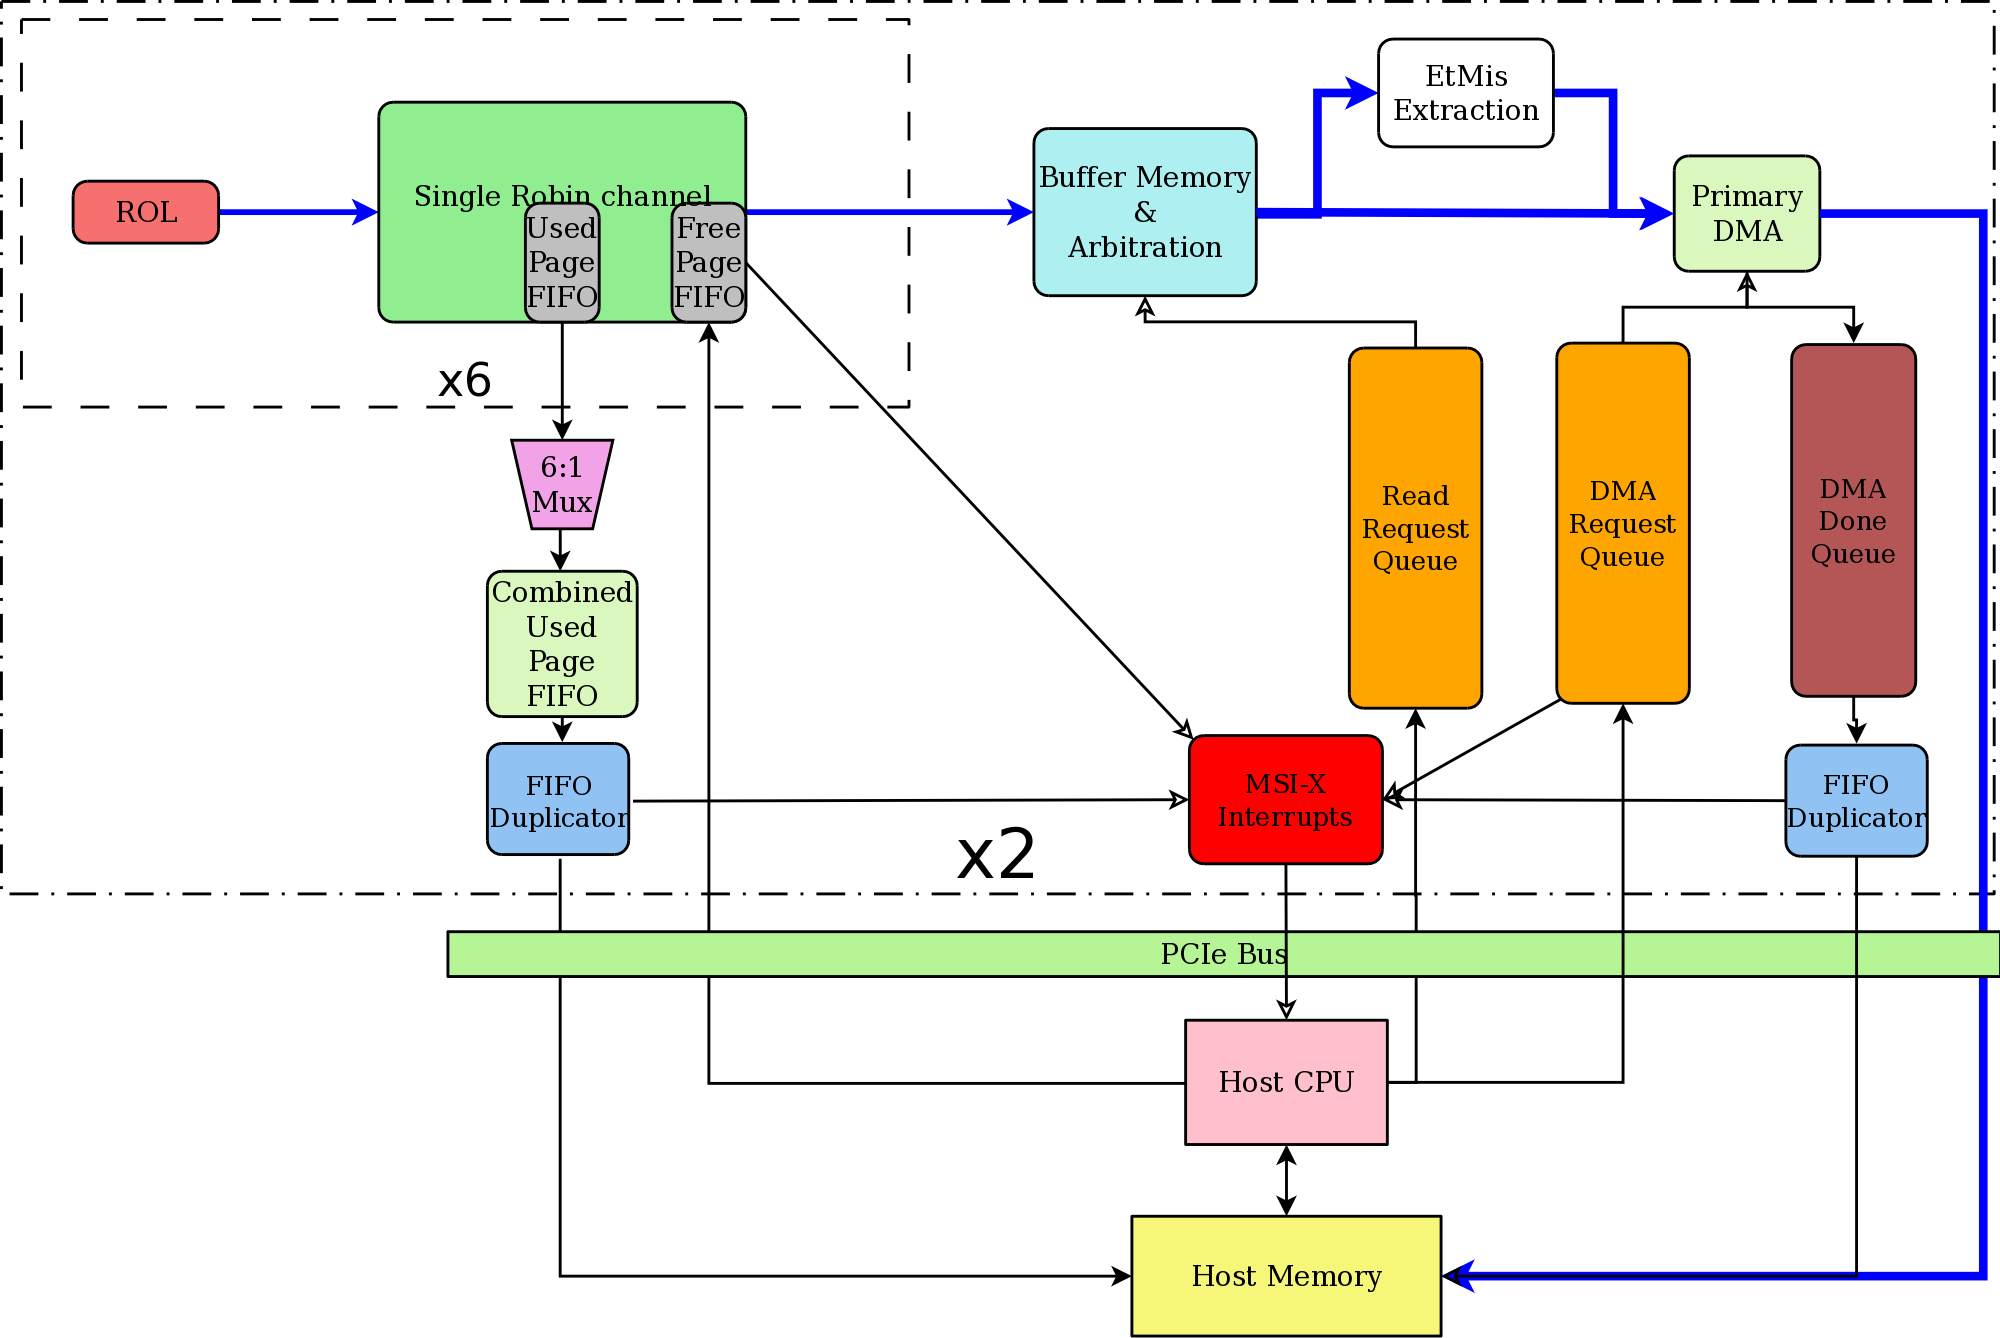
\includegraphics[width=.8\textwidth]{AReducedBlockDiagram.png}

\caption{RobinNP firmware organization
and  flow  of  data  from  host  CPU  to  the
firmware  (by  means  of  programmed  I/O)
and from the firmware to the host memory
(by means of DMA).}
\label{fig:robinnp_fw}
\end{figure}

\subsection{Readout System Firmware \& Software}\label{sec:crorc_fw}

The RobinNP firmware used for the RoIB is identical to that used in the ATLAS ROS\cite{ros}. As shown in 
the schematic of Figure \ref{fig:robinnp_fw}, the logic is divided into two functional blocks, known as sub-ROBs, 
each servicing six input links and one DDR3 memory module. Event data fragments arriving via a link are subjected 
to a range of error checks before being stored in the memory module for the relevant sub-ROB. At the same time a token
representing the address of a region of the memory, referred to as a page, is passed to a listening software process via 
a `FIFO duplicator'. To avoid a costly read across the PCIe bus, data is continuously streamed from firmware to 
software via a chain of firmware and software FIFOs. Notification of new data arriving in the software FIFO is managed via coalesced 
interrupts to allow for efficient use of CPU resources.
For the RoIB application, the receipt of page information immediately triggers a DMA of fragment data from the RobinNP memory into 
the host PC memory. The fragments are then passed via a queue (one per sub-ROB) to the RoIB process along with any relevant fragment 
error information. A schematic of this shortened dataflow path is presented in Figure \ref{fig:roib_swfw}. 
The API for the RoIB process consists of these queues, return queues for processed pages now available for re-use and 
a configuration interface. The software is implemented with multiple threads each handling specific tasks such as supply of free pages, receipt
of used pages, DMA control and bulk receipt of fragment data.


\begin{figure}[tbp] % figures (and tables) should go top or bottom of
                    % the page where they are first cited or in
                    % subsequent pages
\centering
%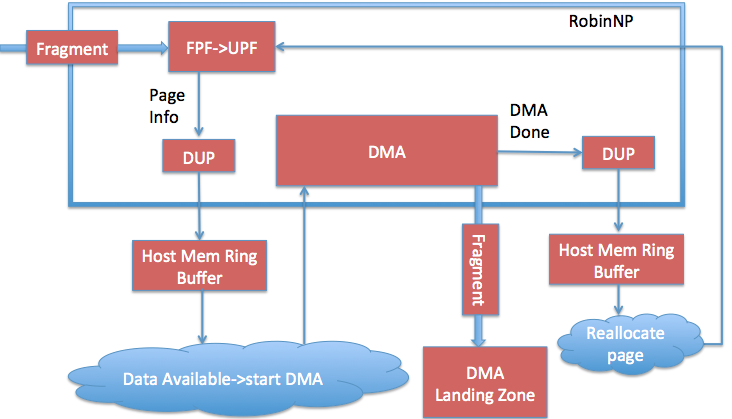
\includegraphics[width=.6\textwidth]{roib_firmware.png}
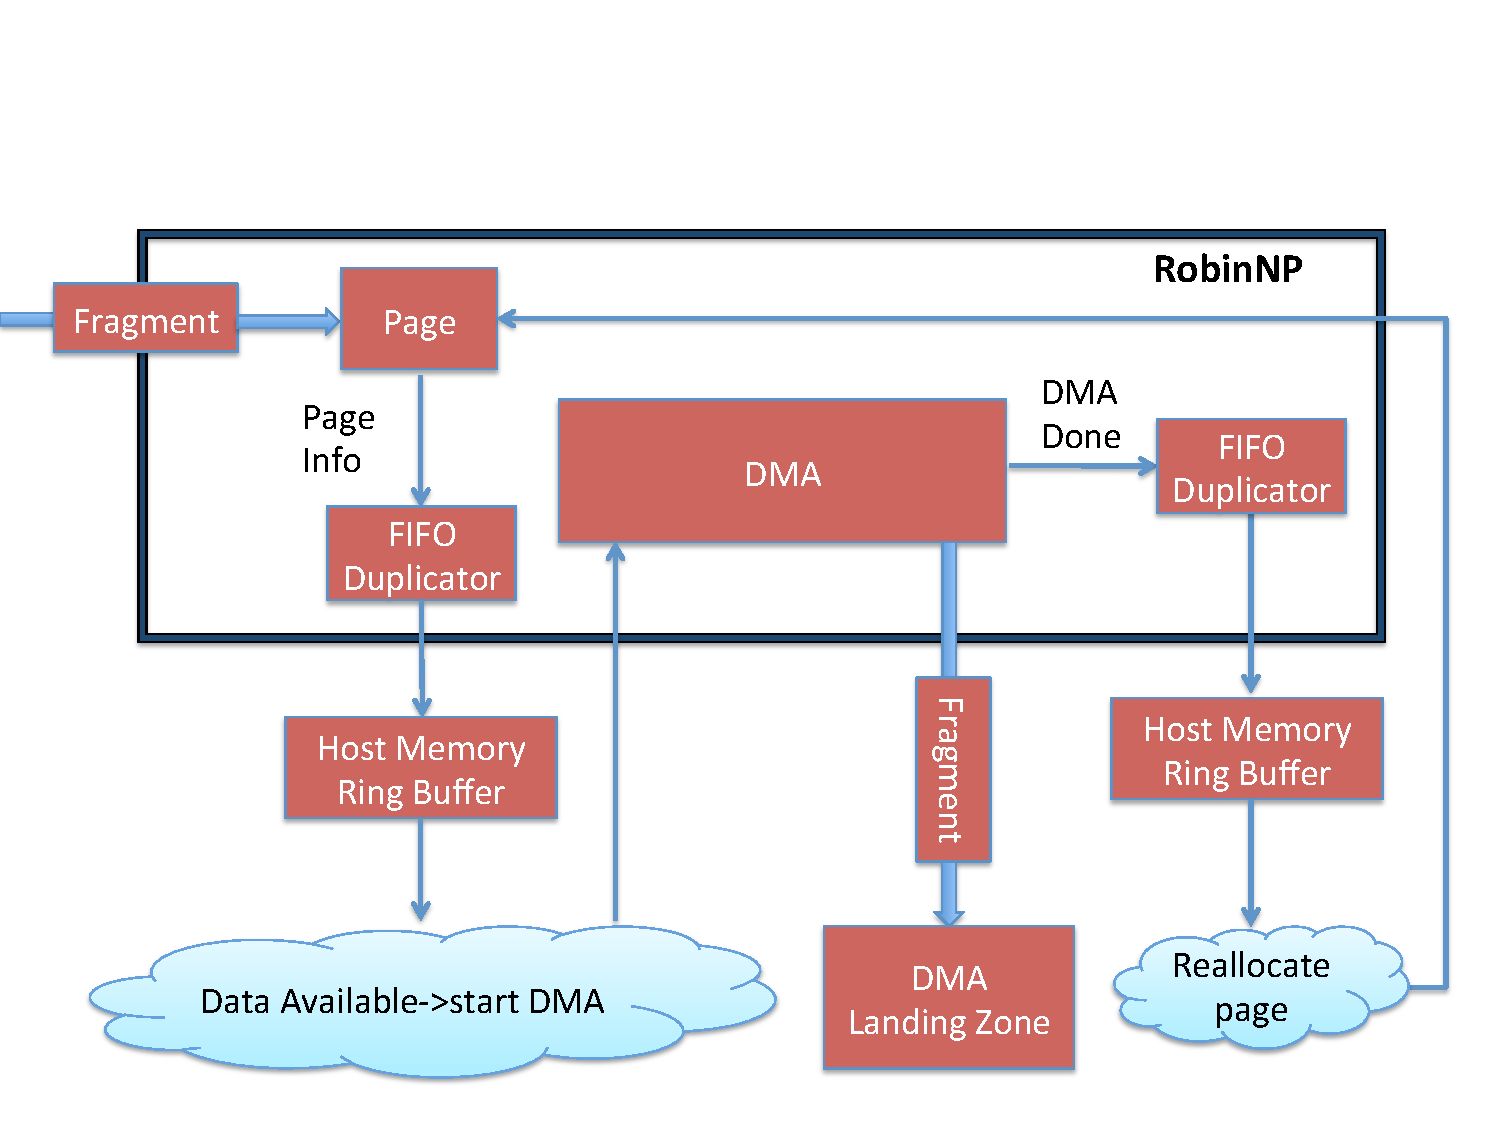
\includegraphics[trim = 0cm 0cm 0cm 5cm, width=.7\textwidth]{RobinNP_Software}
\caption{Layout of the readout system firmware and software specific to the RoIB.}
\label{fig:roib_swfw}
\end{figure}

\subsection{RoIB Software}\label{sec:crorc_sw}

The HLTSV is a multi-threaded application that obtains a L1 result from a variety of possible input sources and exchanges information with the 
rest of the HLT computing farm. 
%Data Collection Managers (DCM). The DCM is the application running on each HLT computing node that tells the HLTSV if the event has been rejected, successfully built, or timed out and also requests the data from the ROS. In this case, 
For the RoIB, the L1 source is a RobinNP interface that performs fragment assembly and is used as a plug-in to the HLTSV application.
The RobinNP plug-in has two receive threads, each 
thread services six channels by pulling fragments from the RobinNP on-board memories to the host PC.
Fragments with the same L1ID are copied 
to a contiguous memory space and a queue of completed events is prepared. 
Upon request by the HLTSV, a pointer to the contiguous memory space is passed back to the 
HLTSV process for further handling. In order to optimize concurrent access to RoIB data structures, containers from the  Intel 
threading building block (TBB) library were used. These containers allow multiple threads to concurrently access and update items 
in the container while maintaining high performance.  


\section{Prototype Tests}\label{sec:perf}

In order to understand the requirements for the underlying server PC, a validation system based on Intel(R) Xeon(R) CPU E5-1650 v2 
@ 3.5 GHz with six cores is being used to perform tests of the PC based RoIB. 
The goal is to perform software based fragment assembly at a rate of 100 kHz over 12 channels for a typical 
fragment size of 400 bytes. The current system offers flexibility in terms of the fragment size allowed which was not the case in the 
VMEbus based RoIB. The initial tests were performed with a standalone application that implements a minimal interface for event building. 
Once the system was validated, the relevant code modules were integrated into an HLTSV process running within the full ATLAS TDAQ 
software suite with appropriately scaled test hardware to represent the remaining elements of the system.

\subsection{Standalone Tests}\label{sec:perf_alone}

The goal was to test input/output bandwidth limitations of the RobinNP and the rate of event building. Initial performance testing used 
a standalone RobinNP application and an external source that emulates the L1 trigger data 
in the form of 32-bit word fragments with 12 channels. In this test, the host PC was running the assembly routine with a single threaded application.  Figure \ref{fig:cern_robinnproib} shows the input rate without 
event building as a function of fragment size. For 400 byte fragments the input rate to the RobinNP is 215 kHz. 
The same figure 
shows the event building rate which is 150 kHz. This performance shows that the event building 
at the required rate of 100 kHz with 12 channels is achievable in a standalone application.  


\begin{figure}[tbp] % figures (and tables) should go top or bottom of
                    % the page where they are first cited or in
                    % subsequent pages
\centering
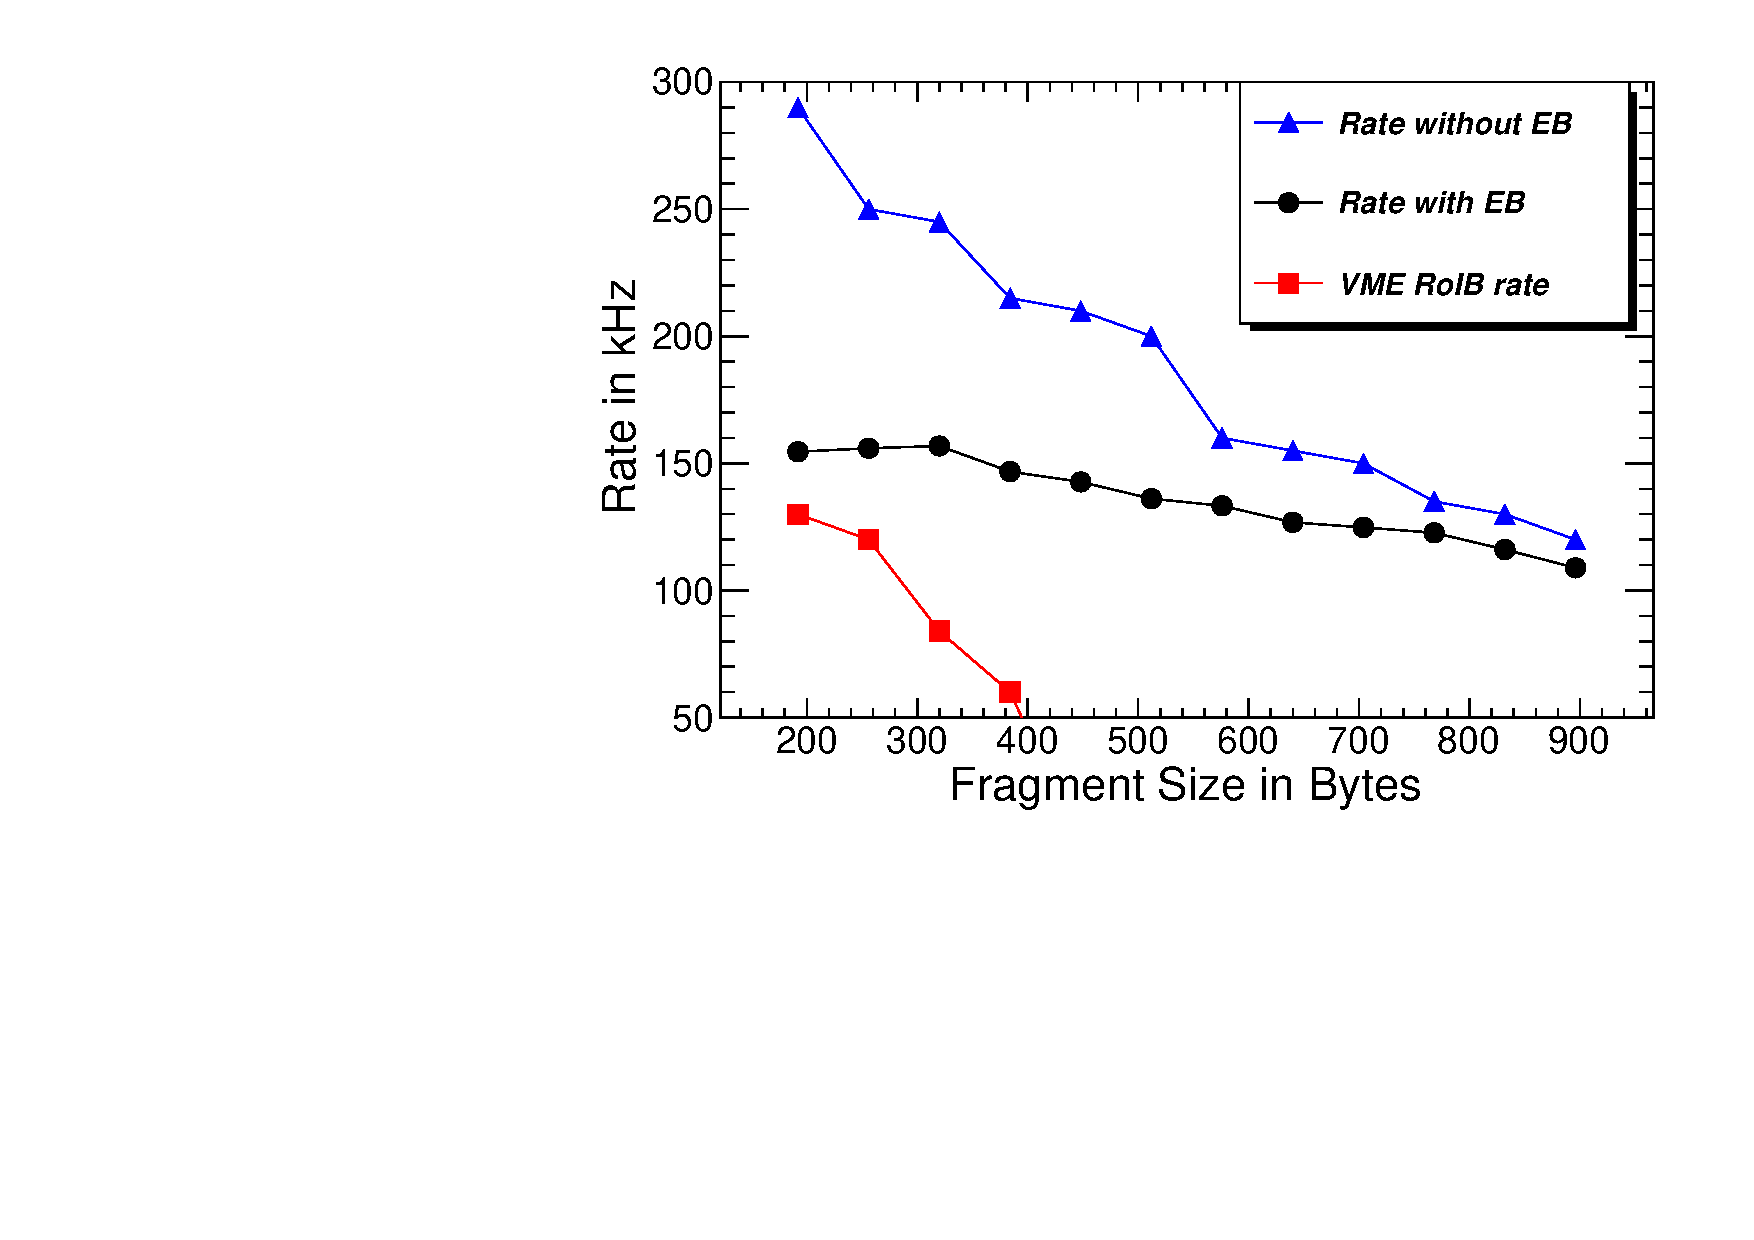
\includegraphics[width=.7\textwidth]{cern_robinnproib.pdf}
\caption{Rate as a function of the fragment size (in bytes) with external source that emulates the L1 trigger input. 
The rates shown are for the input rate to the RobinNP without event building (EB) (triangle), rate with EB (circle), and 
for comparison, the current VMEbus RoIB rate is also shown (square).  }
\label{fig:cern_robinnproib}
\end{figure}


\subsection{Full System Tests}\label{sec:perf_tdaq}

Since the HLTSV is performing tasks other than the event building, there is overhead associated with additional operations 
that reduces the performance. For this reason, we use the full ATLAS TDAQ software in a test environment that emulates the major components of the ATLAS data acquisition system shown in Figure \ref{fig:atlas_tdaq}. The setup includes an emulated input from L1 trigger sources, 
the HLTSV and other PCs to simulate the HLT computing farm, and the ROS that buffers the full event data. 
 In this test setup, an external source sends data that emulates L1 RoIs via 12 links connected to the 
RobinNP hosted by the HLTSV. When the HLTSV requests a built RoI event, the software RoIB plug-in provides the RoI event which will be used 
to seed requests for the event data to be processed.
 Figure \ref{fig:partition} shows an event building rate of 110 kHz measured with 400 byte fragments with the HLTSV application in a setup close to the ATLAS TDAQ system. 

\begin{figure}[tbp] % figures (and tables) should go top or bottom of
                    % the page where they are first cited or in
                    % subsequent pages
\centering
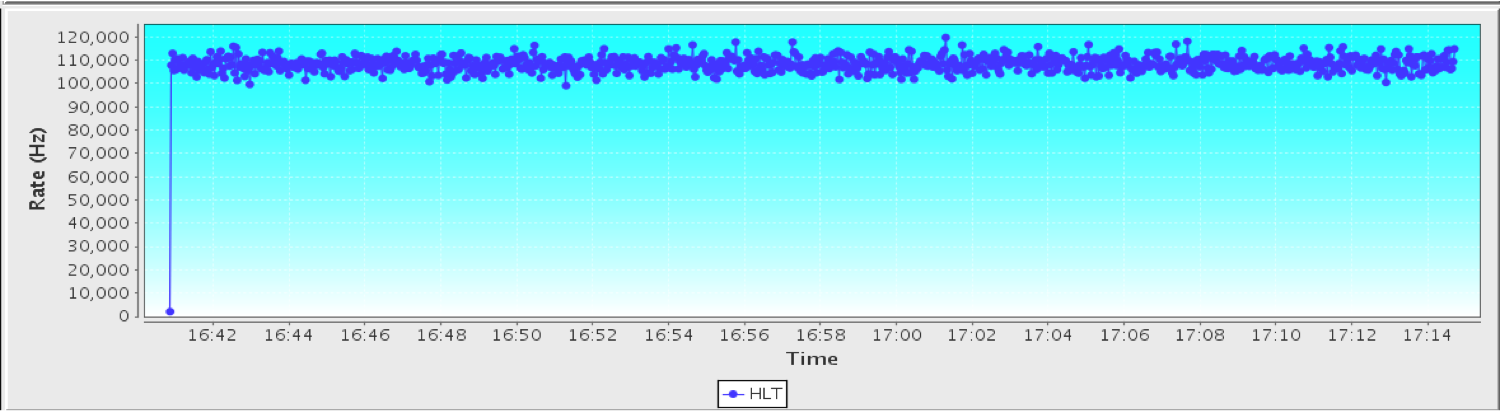
\includegraphics[width=.98\textwidth]{12ch.png}
\caption{Screenshot of a monitoring tool which shows the HLTSV processing rate using the ATLAS TDAQ software .}
\label{fig:partition}
\end{figure}


\section{Outlook}\label{sec:outlook}

The RoIB will evolve from the VMEbus based system to the PC based system using a PCI-Express card and firmware shared with the 
ATLAS ROS. The new system will add flexibility and improve maintainability of the ATLAS TDAQ system. As the technology 
evolves, the PCs and CPUs can be upgraded and more channels can be included by adding more RobinNP cards while maintaining high 
readout rates. A full integration test of the readout performance of the ATLAS TDAQ system with the PC based RoIB will be performed 
during the 2015-2016 LHC winter shutdown in preparation for a system evolution.



%% \bibitem{atlas}
%% ATLAS Collaboration, \emph{The ATLAS experiment at the CERN Large Hadron Collider}, \jinst{3}{2008}{S08003}.

%% \bibitem{evolution}
%%  N. Garelli (on behalf of the ATLAS Collaboration),
%% \emph{The Evolution of the Trigger and Data
%% Acquisition System in the ATLAS Experiment},
%% {J. Phys.: Conf. Ser.
%% 513 (2014) 012007.}



%% \bibitem{l1}
%% ATLAS Collaboration, \emph{ATLAS Level-1 Trigger: Technical Design Report}, 
%% {ATLAS-TDR-12}, 1998


%% \bibitem{hlt}
%% ATLAS Collaboration,
%% \emph{ATLAS, High-Level Trigger, Data Acquisition and Controls} \href{https://cds.cern.ch/record/616089}{https://cds.cern.ch/record/616089}
%% \emph{CERN/LHCC/2003-022}, CERN Geneva 2003.






%% \bibitem{ros}
%% A. Borga et al.,\emph{Evolution of the ReadOut System of the ATLAS experiment}, in proceedings of
%% \emph{Technology and Instrumentation in Particle Physics 2014}, June, 2--6, 2014 Amsterdam, the Netherlands
%% \pos{PoS(TIPP2014)205}.



%% \bibitem{vme_roib}
%% R. Blair et al.,
%% \emph{The ATLAS High Level Trigger Region of Interest Builder},
%% \jinst{3}{2008}{P04001} 


%% \bibitem{swroib_past}
%% R. E. Blair et al., \emph{ATLAS TDAQ dataflow: Software RoI builder status report}, {ATL-DQ-TR-0020}, 2012


%% \bibitem{l1ttc}
%% S. Ask et al., \emph{The ATLAS central level-1 trigger logic and TTC system}, \jinst{3}{2008}{P08002}.

%% \bibitem{tilar}
%% CERN, \url{http://www.cerntech.hu/products/15-tilar-express.html}, October 15, 2015


%% \bibitem{alice}
%% H. Engel,U. Kebschull (For the ALICE Collaboration),
%% \emph{Common read-out receiver card for ALICE Run2},
%% \jinst{8}{2013}{C12016}.

%% \bibitem{crorc}
%% A. Borga et al., \emph{The C-RORC PCIe Card and its Application in the ALICE and ATLAS Experiments}, \jinst{10}{2015}{C02022}.



